\documentclass[12pt,a4 paper]{extreport}
\usepackage{ryan}
\usepackage[bottom]{footmisc}
\usepackage{pdfpages}

\pagestyle{fancy}
\fancyhf{}
\fancyhead[L]{\leftmark}
\fancyhead[R]{\thepage}
\renewcommand{\headrulewidth}{0.4pt}
\renewcommand{\arraystretch}{1.2}
\derivset{\odv}[switch-*=false]

\begin{document}
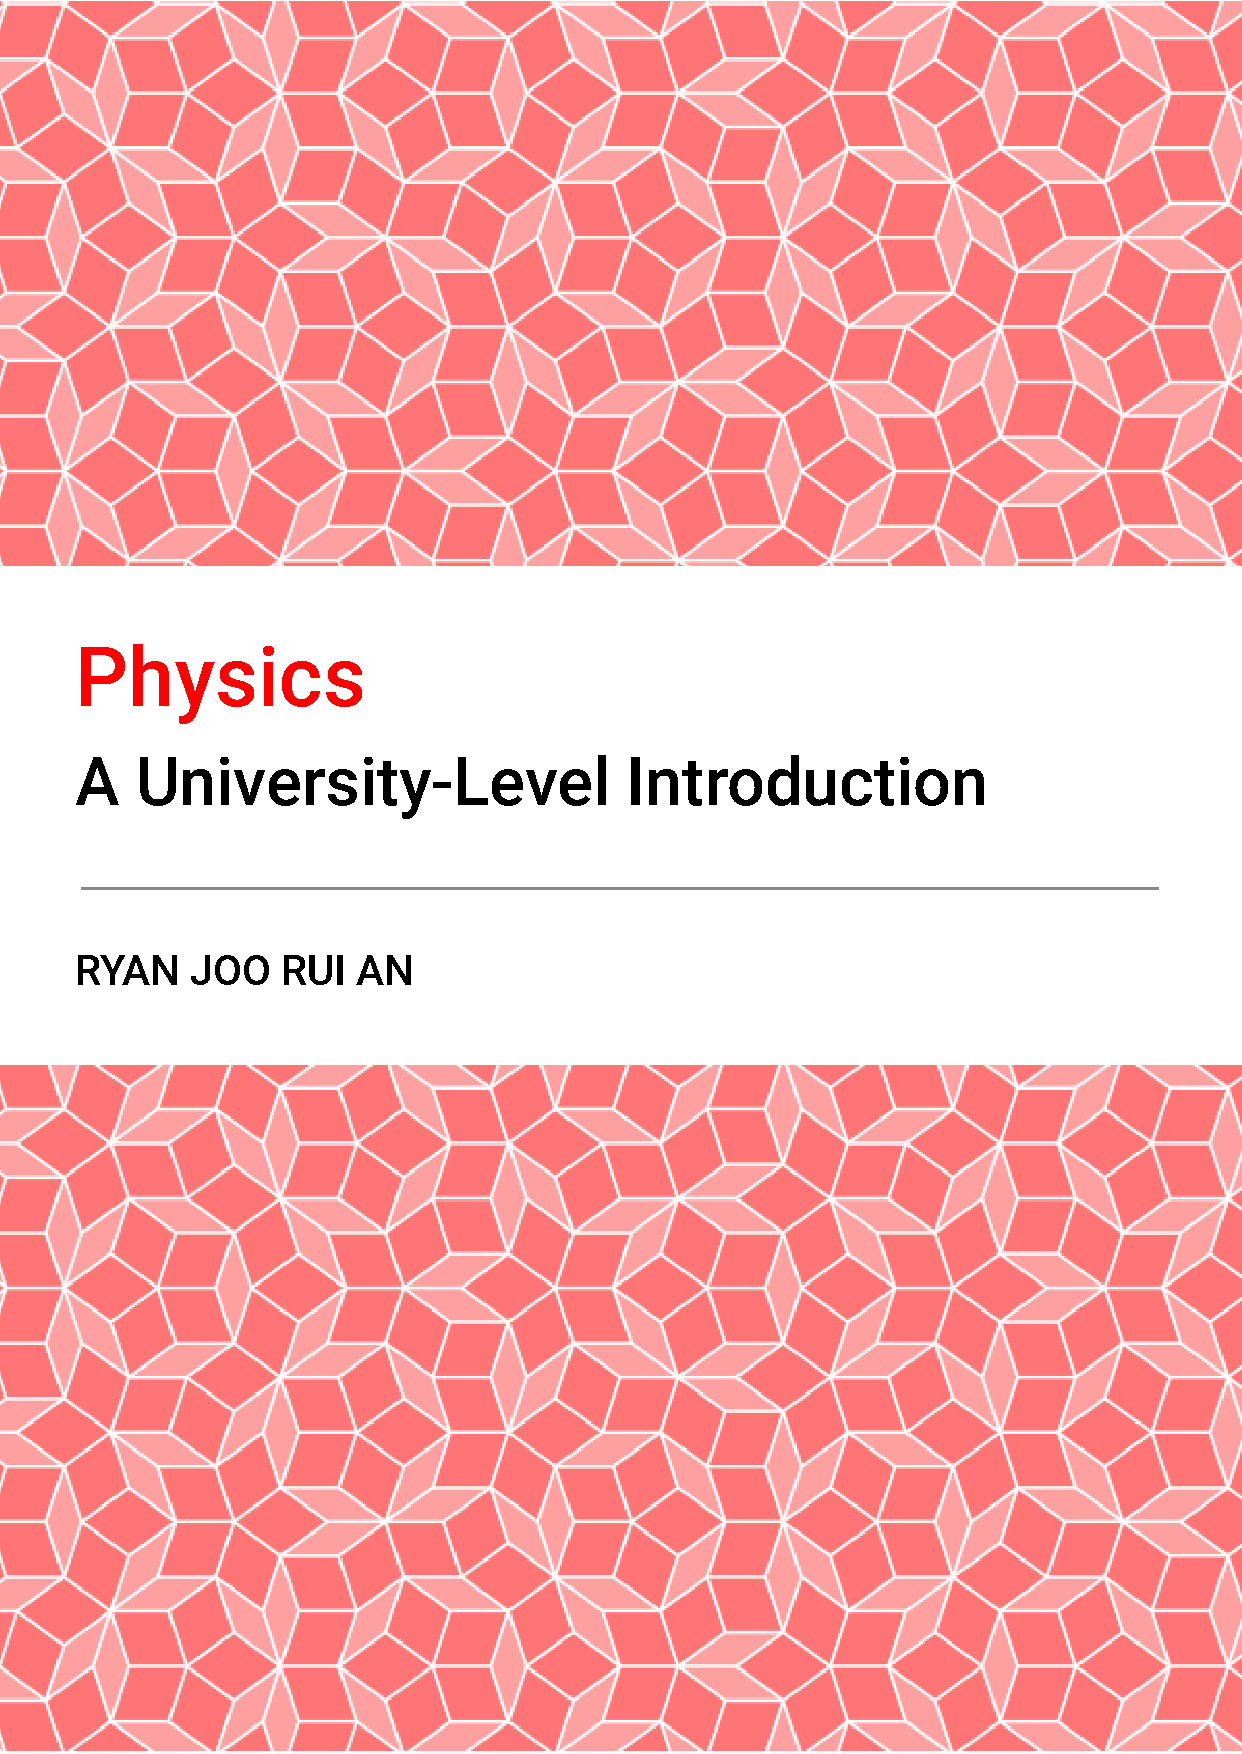
\includepdf{cover_page_phy}
% https://docs.google.com/document/d/1qOQRpuGP99Hcuc8FrVnswpaaACO5ar8KCU8HAPHfC7g/edit?usp=sharing

\begin{titlepage}
\title{Physics:\\
A University-Level Introduction}
\author{Ryan Joo Rui An}
\date{\today}
\end{titlepage}

\maketitle

\chapter*{Preface}
\textbf{Resources:}
\begin{itemize}
\item \href{https://www.geeksforgeeks.org/}{Geeks for Geeks}
\item \href{https://irp-cdn.multiscreensite.com/721e955d/files/uploaded/Physics-Olympiad-Basic-To-Advanced-Exercises.pdf}{Physics Olympiad: Basic to Advanced Exercises}
\item \href{https://knzhou.github.io/}{Kevin Zhou's Physics handouts} % https://knzhou.github.io/notes/phy.pdf
\item \href{https://ocw.mit.edu/}{MIT OpenCourseware}
\item \href{https://www.physicswithelliot.com/all-notes}{Physics with Elliot}
\end{itemize}
% https://docs.google.com/document/d/1CW8sE9ywo62TN0KBZ6tZdhfpyfhgVe2CL6uUotVR1W0/edit
% H3 Physics: https://docs.google.com/document/d/1yMKfgNPBtp0PYMXbVSWEPPSWXL5XQY7plDMGZnue8Is/edit#heading=h.wn92jsim7s8t
% Finish up AP Phy2: https://www.youtube.com/playlist?list=PLoGgviqq4845KrxuxxrWj4WM7oM6Wxl1m

\tableofcontents

\chapter{Mathematics}
\section{Coordinate system}
A vector can be defined in 2 or 3 (or even more) dimensions.

\begin{itemize}
\item Cartesian coordinates

In Cartesian components, the position of a given point $A$ in space is specified by three numbers $(A_x,A_y,A_z)$: $A_x$ is the distance along the $x$-axis, $A_y$ is the distance along the $y$-axis, $A_z$ is the distance along the $z$-axis.

A vector $\vb{A}$ connecting the origin and point $A$ is given by
\[ \vb{A} = A_x\hat{i}+A_y\hat{j}+A_z\hat{k} \]

\item Spherical polar coordinates

The position of a given point in space is specified by three numbers $(r,\theta,\phi)$:
\begin{itemize}
\item $r$: radial distance of the radial line connecting the point to the fixed point of origin
\item $\theta$: polar angle of the radial line, measured between the $z$-axis and the radial line
\item $\phi$: azimuthal angle of the radial line, measured between the orthogonal projection of the radial line $r$ onto the reference $xy$-plane.
\end{itemize}
\end{itemize}




\part{Mechanics}
\chapter{Kinematics}
\section{Uniformly accelerated linear motion}
\subsection{Equations of motion}
\textbf{Velocity} as function of time:
\begin{equation}
v_x(t) = v_{x0} + a_xt
\end{equation}

\begin{derivation}
For the one-dimensional case in the $x$-direction, from the definition of acceleration as the time derivative of velocity,
\[ a_x = \dv{v_x}{t} \]
Solving the differential equation,
\[ \int_{v_{x0}}^{v_x(t)} \dd{v_x} = \int_{0}^{t} a_x \dd{t} \implies v_x(t)-v_{x0} = a_xt \]

$\therefore \vb{v}(t)=(v_{x0}+a_xt)\hat{i}+(v_{y0}+a_yt)\hat{j}$
\end{derivation}

\textbf{Displacement} as function of time:
\begin{equation}
x(t)=x_0+v_{x0}t+\frac{1}{2}a_xt^2
\end{equation}

\begin{derivation}
\begin{align*}
v_x(t) &= \odv{x(t)}{t} \\
v_{x0}+a_xt &= \odv{x(t)}{t} \\
\dd{x} &= (v_{x0}+a_xt) \dd{t} \\
\int_{x_0}^{x(t)} &= \int_0^t (v_{x0}+a_xt) \dd{t} \\
x(t)-x_0 &= v_{x0}t+\frac{1}{2}a_xt^2 \\
x(t) &= x_0+v_{x0}t+\frac{1}{2}a_xt^2
\end{align*}
$\therefore \vb{r}(t)=(x_0+v_{x0}t+\frac{1}{2}a_xt^2)\hat{i}+(y_0+v_{y0}t+\frac{1}{2}a_yt^2)\hat{j}$
\end{derivation}

Eliminating time dependence:
\begin{equation}
v_x(x)^2 = {v_{x0}}^2+2a_x[x(t)-x_0]
\end{equation}

\begin{derivation}
\begin{align*}
a_x(t) &= \odv{v_x(t)}{t} \\
a_x &= \odv{v_x}{x} \odv{x}{t} \\
a_x &= v_x \odv{v_x}{x} \\
a_x \dd{x} &= v_x \dd{v_x} \\
\int_{x_0}^{x(t)}a_x\dd{x} &= \int_{v_{x0}}^{v_x(t)}v_x \dd{v_x} \\
\frac{1}{2}v_x(t)^2 - \frac{1}{2}{v_{x0}}^2 &= a_x[x(t)-x_0] \\
v_x(x)^2 &= {v_{x0}}^2+2a_x[x(t)-x_0] \\
\end{align*}
\end{derivation}

\subsection{Projectile motion}
Horizontal and vertical motions are completely \emph{independent} from each other.

Conventionally, $+x$-direction is horizontally rightward, $+y$-direction is vertically upward.

\begin{table}[H]
\centering
\begin{tabular}{cc}
\hline\hline
\textbf{Horizontal motion} & \textbf{Vertical motion} \\
\hline
$v_x(t)=v_{x0}+a_xt$ & $v_y(t)=v_{y0}+a_yt$ \\
$x(t)=x_0+v_{x0}t+\frac{1}{2}a_xt^2$ & $y(t)=y_0+v_{y0}t+\frac{1}{2}a_yt^2$ \\
$v_x(x)^2={v_{x0}}^2+2a_x(x-x_0)$ & $v_y(y)^2={v_{y0}}^2+2a_y(y-y_0)$ \\
\hline\hline
\end{tabular}
\end{table}

The trajectory of two dimensional free falling motion is given by
\begin{align*}
x(t) &= x_0+v_0\cos\theta t \implies t=\frac{x(t)-x_0}{v_0\cos\theta} \\
y(t) &= y_0+v_0\sin\theta t-\frac{1}{2}gt^2 \\
&= y_0 + \tan\theta[x(t)-x_0]-\brac{\frac{g}{2{v_0}^2\cos^2\theta}}[x(t)-x_0]^2
\end{align*}
Hence, the trajectory is \emph{parabolic}.
\pagebreak

\begin{exmp}{}{}
The acceleration of a marble in a certain fluid is proportional to the speed of the marble squared and is given by $a=-kv^2$. If the marble enters the fluid with a speed of $v_0$, how long will it take before the marble's speed is half of its initial value?
\end{exmp}

\begin{solution}
Rewriting acceleration as the derivative of velocity and solving the differential equation,
\[ a(t) = -kv(t)^2 \implies \dv{v}{t} = -kv^2 \]

Solving the differential equation,
\[ \frac{1}{v^2} \dd{v} = -k \dd{t} \implies
\int_{v_0}^{\frac{v_0}{2}} \frac{1}{v^2} \dd{v} = -\int_0^t k \dd{t} \implies
\frac{2}{v_0} - \frac{1}{v_0} = kt \implies 
\boxed{t = \frac{1}{kv_0}} \]

To determine the displacement of the marble at this time, rewrite acceleration as time derivative of velocity.
\[ \dv{v}{t} = -kv^2 \]
Using chain rule,
\[ \dv{v}{x}\dv{x}{t} = -kv^2 \]
Since $v=\dv{x}{t}$,
\[ v\odv{v}{x} = -kv^2 \]
Solving the differential equation,
\[ \frac{1}{v}\dd{v} = -k \dd{x} \implies
\int_{v_0}^{\frac{v_0}{2}}\frac{1}{v} \dd{v} = -\int_0^xk\dd{x} \implies
\ln\frac{v_0}{2}-\ln v_0 = -kx \implies
\boxed{x = \frac{\ln2}{k}} \]
\end{solution}
\pagebreak

\begin{exmp}{}{}
Ship A is 10km due west of ship B. Ship A is heading directly north at a speed of 30km/h while ship B is heading in a direction 60$\degree$ west of north at a speed of 20km/h. What will be their distance of closest approach?
\end{exmp}

\begin{solution}
We first set up a coordinate system: choose origin at initial position of ship A, $+x$-direction is eastward and $+y$-direction is northward.

Position vector of A with respect to B:
\begin{align*}
\vb{r}_{AB} &= \vb{r}_{AG} + \vb{r}_{GB} \\
&= \vb{r}_{AG} - \vb{r}_{BG} \\
&= v_At\hat{j} + (10-v_Bt\sin60\degree)\hat{i}+v_Bt\cos60\degree\hat{j} \\
&= (-10+v_B\sin60\degree t)\hat{i}+(v_At-v_B\cos60\degree t)\hat{j}
\end{align*}

Relative distance between A and B at time $t$:
\[ r_{AB} = |\vb{r}_{AB}| = \sqrt{(-10+v_B\sin60\degree t)^2+(v_At-v_B\cos60\degree t)^2} \]

To find minimum value of $r_{AB}$,
\[ \dv{r_{AB}}{t}=0 \implies t_0=\frac{\sqrt{3}}{7} \]

$\therefore$ Minimum distance between A and B = \boxed{7.56 \unit{km}}.
\end{solution}
\pagebreak

\begin{exmp}{}{}
A projectile is fired up an incline of angle $\phi$ with an initial speed $v_i$ at an angle $\theta$ with respect to the horizontal ($\theta>\phi$). Find the direction in which it should be aimed to achieve the maximum range along the incline. What is the maximum range?
\end{exmp}

\begin{solution}
$\vb{v}_x(t)=v_i\cos\theta, \vb{v}_y(t)=v_i\cos\theta$
Let the time when projectile lands on the incline be $T$.

\end{solution}
\pagebreak

\begin{exmp}{}{}
At $t=0$ on a planet, a projectile is fired with speed $v_0$ at an angle $\theta$ above the horizontal. On this planet, the acceleration due to gravity increases linearly with time, starting with a value of zero when the projectile is fired from the ground, i.e. $g(t)=\alpha t$. What horizontal distance does the projectile travel? What should $\theta$ be to maximise this distance?
\end{exmp}

\chapter{Newtonian Mechanics}
Classical mechanics is all about the motion of \textbf{particles}. We start with a definition.

\begin{defn}{Particle}{}
A particle is, loosely, defined as an object of insignificant size. 

This means that if you want to say what a particle looks like at a given time, the only information you have to specify is its position.
\end{defn}

To describe the position of a particle we need a \textbf{reference frame}. This is a choice of origin, together with a set of axes which, for now, we pick to be Cartesian. With respect to this frame, the position of a particle is specified by a vector $\vb{x}$. The trajectory of the particle with respect to time is described by
\[ \vb{x}=\vb{x}(t) \]

\begin{notation}
In this book we will use both the notation $\vb{x}(t)$ and $\vb{r}(t)$ to describe the trajectory of a particle.
\end{notation}

\begin{defn}{Velocity}{}
The \vocab{velocity} of a particle is defined to be
\begin{equation}
\vb{v} \equiv \dot{\vb{x}} = \dv{\vb{x}(t)}{t}
\end{equation}
\end{defn}

\begin{notation}
We often denote the time derivative of a variable by a dot above the variable.
\end{notation}

\begin{defn}{Acceleration}{}
The \vocab{acceleration} of the particle is defined to be
\begin{equation}
\vb{a} \equiv \ddot{\vb{x}} = \dv[2]{\vb{x}(t)}{t}
\end{equation}
\end{defn}

\subsection*{Vector Differentiation}
The derivative of a vector is defined by differentiating each of the components. For $\vb{x} = (x_1, x_2, x_3)$,
\[ \dv{\vb{x}}{t} = \brac{\dv{x_1}{t}, \dv{x_2}{t}, \dv{x_3}{t}} \]
Geometrically, the derivative of a path $\vb{x}(t)$ lies tangent to the path.

We will also be working with vector differential equations. These should be viewed as three, coupled differential equations -- one for each component. We will frequently come across situations where we need to differentiate vector dot-products and cross-products. The meaning of these is easy to see if we use the chain rule on each component. For example, given two vector functions of time, $\vb{f}(t)$ and $\vb{g}(t)$, we have
\[ \odv*{(\vb{f}\cdot\vb{g})}{t} = \dv{\vb{f}}{t}\cdot \vb{g}+\vb{f}\cdot\dv{\vb{g}}{t} \]
and
\[ \odv*{(\vb{f}\times\vb{g})}{t} = \dv{\vb{f}}{t}\times\vb{g}+\vb{f}\times\dv{\vb{g}}{t} \]

Note that the order that we write the dot product does not matter, but we have to be more careful with the cross product because, for example, 
\[ \dv{\vb{f}}{t} \times \vb{g} = -\vb{g} \times \dv{\vb{f}}{t}. \]

\section{Newton's Laws}
Newtonian mechanics is a framework which allows us to determine the trajectory $\vb{x}(t)$ of a particle in any given situation. This framework is usually presented as three axioms known as \vocab{Newton's laws of motion}. They are given by:
\begin{enumerate}[label=\textbf{N\arabic*}]
\item Left alone, a particle moves with constant velocity.
\item The acceleration (or, more precisely, the rate of change of momentum) of a particle is proportional to the force acting upon it.
\item Every action has an equal and opposite reaction.
\end{enumerate}

\section{Inertial Frames and Newton's First Law}
We have introduced the idea of a frame of reference: a Cartesian coordinate system in which you measure the position of the particle. But for reference frames such as rotating ones, for a particle of trajectory $\vb{x}(t)$, we certainly won't find that $d^2\vb{x}/dt^2=0$, i.e. particles do not travel at constant velocity.

We see that if we want Newton's first law to hold, we must be more careful about the kind of reference frames we're talking about. We first define an inertial reference frame.

\begin{defn}{Inertial reference frame}{}
An \vocab{inertial reference frame} is one in which particles travel at constant velocity when the force acting on it vanishes. 

In other words, in an inertial frame,
\[ \ddot{\vb{x}}=0 \quad \text{when} \quad \vb{F}=0 \]
\end{defn}

The true content of Newton's first law can then be better stated as: inertial frames exist.

\subsection{Galilean Relativity}
Inertial frames are not unique. Given an inertial frame $S$ in which a particle has coordinates $\vb{x}(t)$, we can always construct another inertial frame $S^\prime$ in which the particle has coordinates $\vb{x}^\prime(t)$ by any combination of the following transformations:
\begin{itemize}
\item Translation: $\vb{x}^\prime = \vb{x} + \vb{a}$, for constant $\vb{a}$.
\item Rotation: $\vb{x}^\prime = \mathbf{R}\vb{x}$, for a $3\times3$ matrix $\mathbf{R}$ obeying $\mathbf{R}^T\mathbf{R}=1$. (This also allows for reflections if $\det\mathbf{R}=-1$, although our interest will primarily be on continuous transformations).
\item Boost: $\vb{x}^\prime = \vb{x} + \vb{v}t$, for constant velocity $\vb{v}$.
\end{itemize}

\begin{remark}
The three transformations above are not quite the unique transformations that map between inertial frames. But, for most purposes, they are the only interesting ones! The others are transformations of the form $\vb{x}^\prime=\lambda\vb{x}$ for some $\lambda\in\RR$. This is just a trivial rescaling of the coordinates; for example, we can measure distances in $S$ in units of metres and distances in $S^\prime$ in units of parsecs.
\end{remark}

It is simple to prove that all of these transformations map one inertial frame to another. Suppose that a particle moves with constant velocity with respect to frame $S$, so that $d^2\vb{x}/dt^2=0$. Then, for each of the transformations above, we also have $d^2\vb{x}^\prime/dt^2=0$ which tells us that the particle also moves at constant velocity in $S^\prime$. Or, in other words, if S is an inertial frame then so too is $S^\prime$. The three transformations generate a group known as the \emph{Galilean group}.

We have already mentioned that Newton's second law is to be formulated in an \textit{inertial frame}. But, importantly, it doesn't matter which inertial frame. In fact, this is true for all laws of physics: they are the same in any inertial frame. This is known as the \textbf{principle of relativity}.

So position, direction and velocity are relative. But acceleration is not. You do not have to accelerate relative to something else. It makes perfect sense to simply say that you are accelerating or you are not accelerating. In fact, this brings us back to Newton's first law: if you are not accelerating, you are sitting in an inertial frame.

\subsection{Absolute Time}
There is one last issue that we have left implicit in the discussion above: the choice of time coordinate $t$. If observers in two inertial frames $S$ and $S^\prime$ fix the units -- seconds, minutes, hours -- in which to measure the duration time then the only remaining choice they can make is when to start the clock. In other words, the time variable in $S$ and $S^\prime$ differ only by
\[ t^\prime = t + t_0 \]

This is sometimes included among the transformations that make up the Galilean group.

The existence of a uniform time, measured equally in all inertial reference frames, is referred to as \textbf{absolute time}. It is something that we will have to revisit when we discuss special relativity. As with the other Galilean transformations, the ability to shift the origin of time is reflected in an important property of the laws of physics. The fundamental laws don't care when you start the clock. All evidence suggests that the laws of physics are the same today as they were yesterday. They are \textbf{time translationally invariant}.

\section{Newton's Second Law}
The second law is the meat of the Newtonian framework. It is the famous ``$F=ma$", which tells us how a particle's motion is affected when subjected to a force $\vb{F}$. The
correct form of the second law is
\begin{equation}
\odv*{(m\dot{\vb{x}})}{t} = \vb{F}(\vb{x},\dot{\vb{x}})
\end{equation}
This is usually referred to as the equation of motion. The quantity in brackets is called the \vocab{momentum}:
\[ \vb{p} \equiv m\dot{\vb{x}} \]
where $m$ is the (inertial) mass of the particle.

In cases where mass does not change with time, we can write the second law in the more familiar form:
\begin{equation}
m\ddot{\vb{x}} = \vb{F}(\vb{x},\dot{\vb{x}})
\end{equation}

Newton's equation is a second order differential equation; this means that we will have a unique solution only if we specify two initial conditions. These are usually taken to be the position $\vb{x}(t_0)$ and the velocity $\dot{\vb{x}}(t_0)$ at some initial time $t_0$.

\chapter{Forces}
\section{Potentials in One Dimension}
Consider a particle with position function $x(t)$. For now, suppose that the force on the particle depends only on its position, not its velocity: $F=F(x)$. We define the \vocab{potential} $V(x)$ (also called the potential energy) by the equation
\begin{equation}\label{potential}
F(x) = -\dv{V}{x}
\end{equation}

The potential is only defined up to an additive constant. We can always invert \cref{potential} by integrating both sides. The integration constant is now determined by the choice of lower limit of the integral:
\[ V(x) = -\int_{x_0}^x F(x^\prime) \dd{x^\prime} \]
where $x^\prime$ is just a dummy variable.

With this definition, we can write the equation of motion as
\begin{equation}\label{conservative}
m\ddot{x} = -\dv{V}{x}
\end{equation}

For any force in one-dimension which depends only on the position, there exists a \emph{conserved} quantity called the \vocab{energy},
\[ E = \frac{1}{2}m\dot{x}^2 + V(x) \]

The fact that this is conserved means that $\dot{E} = 0$ for any trajectory of the particle which obeys the equation of motion. While $V(x)$ is called the potential energy, $T=\frac{1}{2}m\dot{x}^2$ is called the \vocab{kinetic energy}. Motion satisfying \cref{conservative} is called \vocab{conservative}.

It is not hard to prove that $E$ is conserved. We need only differentiate with respect to time to get
\[ \dot{E} = m\dot{x}\ddot{x} + \dv{V}{x}\dot{x} = \dot{x}\brac{m\ddot{x}+\dv{V}{x}} = 0 \]
where the last equality holds courtesy of the equation of motion \cref{conservative}.

\subsection{Uniform Gravitational Field}
In a uniform gravitational field, a particle is subjected to a constant force, $F=-mg$ where $g \approx 9.8$  \unit{ms^{-2}} is the acceleration due to gravity near the surface of the Earth. The minus sign arises because the force is downwards while we have chosen to measure position in an upwards direction, which we call $z$. The potential energy is
\begin{equation}
V = mgz
\end{equation}

\begin{remark}
Notice that we have chosen to have $V=0$ at $z=0$. There is nothing that forces us to do this; we could easily add an extra constant to the potential to shift the zero to some other height.
\end{remark}

The equation of motion for uniform acceleration is
\[ \ddot{z}=-g \]
Which can be integrated to give the velocity at time $t$,
\[ \dot{z} = u - gt \]
where $u$ is the initial velocity at time $t=0$.

Integrating once more gives the position
\[ z = z_0 + ut - \frac{1}{2}gt^2 \]
where $z_0$ is the initial height at time $t=0$.

\subsection{Harmonic Oscillator}
The potential energy of the harmonic oscillator is defined to be
\[ V(x) = \frac{1}{2}kx^2 \]

The force resulting from the energy $V$ is given by $F=-kx$ which, in the context of the spring, is called \vocab{Hooke's law}. The equation of motion is
\begin{equation}
m\ddot{x} = -kx
\end{equation}
which has the general solution
\[ x(t) = A \cos(\omega t) + B \sin(\omega t) \quad \text{with }\omega=\sqrt{\frac{k}{m}} \]
where $A$ and $B$ are two integration constants and $\omega$ is called the angular frequency. The coefficients $A$ and $B$ determine the amplitude of the oscillations, together with the phase at which you start the cycle. The time taken to complete a full cycle is called the period
\begin{equation}
T = \frac{2\pi}{\omega}
\end{equation}
The period is independent of the amplitude.

If we want to determine the integration constants A and B for a given trajectory, we need some initial conditions. For example, if we're given the position and velocity at time $t=0$, then it's simple to check that $A=x(0)$ and $B=\frac{\dot{x}(0)}{\omega}$.

\subsection{Moving in a Potential}


\chapter{Translational Dynamics}
\section{Forces}
\subsection{Types of forces}
\subsubsection{Weight}
Weight $\vb{W}$ is the gravitational force exerted by Earth on an object.

\subsubsection{Normal force}
Normal force $\vb{N}$ is the contact force exerted by a surface (ground or floor) on an object.

\subsubsection{Tension force}
Tension force $\vb{T}$ is the force experienced in an object when it is deformed (compressed or depressed).

\subsubsection{Spring force}
\begin{thrm}{Hooke's Law}{}
Spring force is directly proportional to extension of spring.
\begin{equation}
\vb{F}_s = -k\vb{x}
\end{equation}
where $k$ is the spring constant.
\end{thrm}

\subsubsection{Frictional force}
There are two types of frictional force:
\begin{itemize}
\item \textbf{Kinetic friction force}: object is sliding on rough surface
\[ f_k = \mu_k N \]
\item \textbf{Static friction force}: object is not sliding
\[ f_s \le \mu_s N \]
\end{itemize}

\subsubsection{Resistive force}
Drag force $F_R$: force caused by interaction of an object and the fluid it is moving through
\begin{itemize}
\item For objects moving at low speeds: resistive force is directly proportional to speed
\begin{equation}
\vb{F}_R = -b\vb{v}
\end{equation}

\item For objects moving at high speeds: resistive force is directly proportional to square of speed
\begin{equation}
\vb{F}_R = -\frac{1}{2}D\rho A\vb{v}^2
\end{equation}
where $D$ is the drag coefficient, which depends on the shape and surface texture of the object.

\textbf{Terminal velocity} is when an object moving through a fluid has reached translational equilibrium. For an object falling downwards:
\[ \sum \vb{F}_y = \vb{F}_g-\vb{F}_R = m\vb{a}_y \implies mg-\frac{D}{\rho}Av^2 = ma_y \implies a_y = g-\frac{D\rho Av^2}{2m} \]
In absence of air resistance, $\vb{a}_y=g$.

When $\vb{a}_y=0$,
\[ \frac{D\rho Av^2}{2m} = g \implies \boxed{v_\text{terminal} = \sqrt{\frac{2mg}{D\rho A}}} \]
\end{itemize}
\pagebreak

\section{Centre of mass}
\begin{defn}{Centre of mass}{}
A special point in a system, as if all of the mass of the system is concentrated at that point. 
\end{defn}

Centre of mass for a \textbf{system of point particles}:
\begin{equation}
x_{CM} = \frac{\sum_i m_i x_i}{\sum_i m_i} \quad 
y_{CM} = \frac{\sum_i m_i y_i}{\sum_i m_i} \quad
z_{CM} = \frac{\sum_i m_i z_i}{\sum_i m_i}
\end{equation}
where the distances depend on the \emph{coordinate system} set up.

Centre of mass of an \textbf{extended object} (think of an extended object as a system containing infinitely many small mass elements):
\[ x_{CM} = \lim_{\Delta m_i \to 0} \frac{1}{M} \sum_i x_i \Delta m_i \]
\begin{equation}
x_{CM} = \frac{1}{M} \int x \dd{m} \quad
y_{CM} = \frac{1}{M} \int y \dd{m} \quad
z_{CM} = \frac{1}{M} \int z \dd{m}
\end{equation}

\subsection{Motion of centre of mass}
\subsubsection{Velocity}
$x$-, $y$- and $z$-components of the velocity of centre of mass, denoted by $v_{CM,x}$, $v_{CM,y}$ and $v_{CM,z}$, are the time derivatives of $x_{CM}$, $y_{CM}$ and $z_{CM}$ respectively.
\begin{equation}
v_{CM,x} = \frac{\sum_i m_i v_{xi}}{\sum_i m_i} \quad 
v_{CM,y} = \frac{\sum_i m_i v_{yi}}{\sum_i m_i} \quad
v_{CM,z} = \frac{\sum_i m_i v_{zi}}{\sum_i m_i}
\end{equation}

These equations can be written as one single vector equation:
\begin{equation}
\vb{v}_{CM} = \frac{1}{M}\sum_{i}m_i\vb{v}_i
\end{equation}

Total momentum of the system is given by
\begin{equation}
\vb{p} = M\vb{v}_{CM} = \sum_{i}m_i\vb{v}_i
\end{equation}
This equation states that the total momentum is the product of total mass and velocity of centre of mass.

\subsubsection{Acceleration and external force}
Taking time derivative of the above equation gives
\[ M\vb{a}_{CM} = \sum_{i}m_i\vb{a}_i \]

Note that $\sum_{i}m_i\vb{a}_i$ is simply the sum of all forces (external and internal):
\[ \sum\vb{F} = \sum\vb{F}_{ext} + \sum\vb{F}_{int} = \sum_{i}m_i\vb{a}_i \]

By Newton's 3rd law, internal forces all cancel in pairs so $\sum\vb{F}_{int}=0$. Hence
\begin{equation}
\sum\vb{F}_{ext} = M\vb{a}_{CM} \quad \text{and} \quad \sum\vb{F}_{ext}=\odv{\vb{p}}{t}
\end{equation}

When a body or a collection of particles is acted on by external forces, centre of mass moves as though all the mass were concentrated at that point and it were acted on by a net force equal to the sum of external forces on the system.

For example, a shell explodes into two fragments in flight. Ignoring air resistance, centre of mass continues on the same trajectory aas the shell's path before exploding.
\begin{figure}[H]
    \centering
    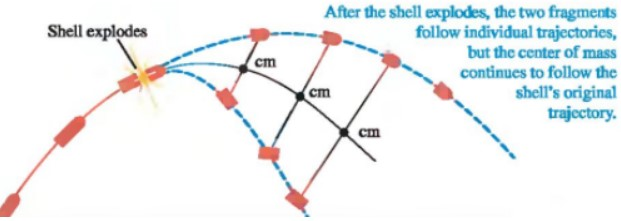
\includegraphics{images/shell_explode_cm.jpg}
\end{figure}

Note that if the net external force acting on the system is zero, we get
\[ \dv{\vb{p}}{t}=0 \implies M\vb{v}_{CM}=\vb{p}=\text{constant} \]
\pagebreak

\section{Equilibrium}
Equilibrium conditions: 
\begin{enumerate}
\item force balance (vectorially or in terms of projections)
\item torque balance (only for one- and two-dimensional geometry). 
\end{enumerate}

Stable and unstable equilibria.
\pagebreak

\section{Elastic modulus}
compression.
We consider three types of deformation and define an elastic modulus for each:
\begin{enumerate}
\item \textbf{Young's modulus} measures the resistance of a solid to a change in its length.
\item \textbf{Shear modulus} measures the resistance to motion of the planes within a solid parallel to each other.
\item \textbf{Bulk modulus} measures the resistance of solids or liquids to changes in their volume.
\end{enumerate}

\subsection{Tensile and compressive}
We usually assume objects to be rigid. When large forces are applied to an object, it deforms. 

Suppose that we pull on the ends of a bar with a force $F$. We say that the bar is in tension. The internal forces in the bar resist the tension forces and hold the bar together. Even so, the bar deforms and the equilibrium length of the bar increases. 

If the bar is in equilibrium with the applied forces, then every cross section of the bar must be subject to the same internal forces that resist stretching.

\begin{defn}{Stress}{}
Ratio of the magnitude of the applied force $F$ to cross-sectional area $A$.
\begin{equation}
\sigma \equiv \frac{F}{A}
\end{equation}
\end{defn}

\begin{remark}
There are two types of stress: tensile and compressive.
\end{remark}

\begin{defn}{Strain}{}
Ratio of the change in length $\delta$ to the initial length $L$.
\begin{equation}
\varepsilon \equiv \frac{\delta}{L}
\end{equation}
\end{defn}

\begin{remark}
There are two types of strain: tensile and compressive.
\end{remark}

The amount of strain an object undergoes depends on the stress applied to it. If the stress is not too great, the strain is observed to be proportional to the stress.

\begin{defn}{Young modulus}{}
Ratio of stress to strain.
\begin{equation}
Y \equiv \frac{\sigma}{\varepsilon} = \frac{FL}{A\delta}
\end{equation}
\end{defn}

\subsection{Shear}
When an external force acts on an object, it undergoes deformation. If the direction of the force is parallel to the plane of the object. The deformation will be along that plane. The stress experienced by the object here is shear stress.

\begin{defn}{Shear stress}{}
A type of stress that acts coplanar with cross section of material.
\begin{equation}
\tau \equiv \frac{F}{A}
\end{equation}
\end{defn}

Shear stress arises due to shear forces. They are the pair of forces acting on opposite sides of a body with the same magnitude and opposite direction. 
\pagebreak

\section{Work Done and Energy}
\subsection{Work}
Work done by a constant force:
\begin{equation}
W = \vb{F} \cdot \Delta\vb{r} = F\Delta r\cos\theta
\end{equation}
where $\theta$ is the angle between $\vb{F}$ and $\vb{r}$.

Work done by a non-constant force:
\begin{equation}
W = \int_{x_i}^{x_f}F_x \dd{x}
\end{equation}

\subsection{Energy}
\begin{thrm}{Net Work -- Kinetic Energy Theorem}{}
\begin{equation}
\sum W = \Delta K
\end{equation}
\end{thrm}

Kinetic energy for translational motion:
\begin{equation}
K=\frac{1}{2}mv^2
\end{equation}

Gravitational potential energy (in constant gravitational field):
\begin{equation}
U_g = mgh
\end{equation}

Potential energy for simple force fields (also as a line integral of the force field). 


Relationship between conservative forces and potential energy:
\begin{equation}
F = -\dv{U}{x}
\end{equation}


\subsection{Power}
\begin{defn}{Power}{}
Rate at which work is done
\begin{equation}
P_\text{avg} = \frac{W}{\Delta t}
\end{equation}
\begin{equation}
P_\text{instantaneous} = \dv{W}{t}
\end{equation}
\end{defn}

Instantaneous power (constant force):
\begin{equation}
P_\text{instantaneous} = \vb{F} \cdot \vb{v}
\end{equation}
\begin{derivation}
\[ P_\text{instantaneous} = \dv{W}{t} = \dv{(\vb{F}\cdot\Delta\vb{r})}{t} = F \cdot \dv{\Delta\vb{r}}{t} = \vb{F}\cdot\vb{v} \]
\end{derivation}

\pagebreak

\chapter{Rotational Motion}
\section{Kinematics}
\begin{defn}{Radian}{}
\begin{equation}
\theta \equiv \frac{s}{r}
\end{equation}
\end{defn}

\begin{defn}{Angular displacement}{}
The angle that a rigid object rotates through during some time interval.
\begin{equation}
\Delta \theta \equiv \theta_f - \theta_i
\end{equation}
\end{defn}

\begin{remark}
Every point on a rigid object undergoes the same angular displacement in any given time interval.
\end{remark}

\begin{defn}{Angular velocity}{}
Rate of change of angular displacement with respect to time.
\begin{equation}
\omega(t) \equiv \lim_{\Delta t \to 0} \frac{\Delta \theta}{\Delta t} = \dv{\theta (t)}{t}
\end{equation}
\end{defn}

\begin{remark}
Every part of a rotating rigid object has the same angular velocity at any instant of time.
\end{remark}

Direction of angular velocity can be found using the ``right hand rule". Curl fingers of right hand around rotation. Thumb points in the direction of the vector.

\begin{defn}{Angular acceleration}{}
Rate of change of angular velocity with respect to time.
\begin{equation}
\alpha (t) \equiv \lim_{\Delta t \to 0} \frac{\Delta \omega}{\Delta t} = \odv{\omega (t)}{t} = \odv{^2 \theta (t)}{t}
\end{equation}
\end{defn}

\textbf{Angular velocity} as a function of time 
\begin{equation}
\omega(t) = \omega_0 + \alpha t
\end{equation}

\textbf{Angular position} as a function of time
\begin{equation}
\theta(t) = \theta_0 + \omega_0 t + \frac{1}{2}\alpha t^2
\end{equation}

Eliminating time dependence
\begin{equation}
\omega^2(t) = {\omega_0}^2 + 2 \alpha [\theta (t) - \theta_0]
\end{equation}

For constant $a$ and $\alpha$, we can write analogous equations for rotational motion as in linear motion, as shown above.

\textbf{Tangential velocity} (linear speed):
\begin{equation}
v = r\omega
\end{equation}

\begin{derivation}
\[ v = \odv{s}{t} = \odv{(r\theta)}{t} = r\odv{\theta}{t} = r\omega \]
\end{derivation}

\textbf{Tangential acceleration}:
\begin{equation}
a_t = r \alpha
\end{equation}
\begin{derivation}
\[ a_t = \odv{v}{t} = \odv{(r\omega)}{t} = r\odv{\omega}{t} = r\alpha \] 
\end{derivation}

\textbf{Centripetal acceleration}
\begin{equation}
a_r = \frac{v^2}{r} = r\omega^2
\end{equation}
\begin{derivation}
\begin{align*}
\frac{\Delta v}{v} &= \frac{\Delta s}{r} \\
\Delta v &= \frac{v}{r} \Delta s \\
\lim_{\Delta t \to 0} \frac{\Delta v}{\Delta t} &= \frac{v}{r} \lim_{\Delta t \to 0} \frac{\Delta s}{\Delta t}
\end{align*}
\end{derivation}

Acceleration is the vector sum of tangential acceleration and centripetal acceleration.
\[ \vb{a} = \vb{a_t} + \vb{a_r} \]
\begin{equation}
|\vb{a}| = \sqrt{{a_t}^2 + {a_r}^2} = r \sqrt{\alpha^2 + \omega^4}
\end{equation}

Comparison between translational and rotational motion:
\begin{table}[H]
\centering
\begin{tabular}{|c|c|c|}
\hline
Quantity & Translational & Rotational \\
\hline
Displacement & $x$ & $\theta$ \\
Velocity & $v$ & $\omega$ \\
Acceleration & $a$ & $\alpha$ \\
Mass / moment of inertia & $m$ & $I$ \\
Momentum & $p$ & $L$ \\
\hline
\end{tabular}
\end{table}
\pagebreak

\section{Dynamics}
\subsection{Moment of Inertia}
Moment of inertia is the measure of the resistance of an object to changes in its rotational motion, depends on the \underline{choice of rotational axis}.

Moment of inertia of one particle:
\begin{equation}
I \equiv mr^2
\end{equation}

Moment of inertia of a system of particles:
\begin{equation}
I = \sum_i m_i {r_i}^2
\end{equation}

Moment of inertia of a continuous rigid object (divide it into infinitely many small elements):
\[ I = \lim_{\Delta m_i \to 0} \sum_i {r_i}^2 \Delta m_i \]
\begin{equation}
I = \int r^2 \dd{m}
\end{equation}

Moments of inertia of homogeneous rigid objects:\footnote{Memorise these important ones.}
\begin{table}[H]
\centering
\renewcommand{\arraystretch}{2.0}
\begin{tabular}{|c|c|}
\hline
\textbf{Object} & \textbf{Moment of inertia} \\
\hline
Hoop about central axis & $I=MR^2$ \\
Solid cylinder (or disk) about central axis & $I=\dfrac{1}{2}MR^2$ \\
Solid cylinder (or disk) about central diameter & $I=\dfrac{1}{4}MR^2+\dfrac{1}{12}ML^2$ \\
Thin rod about axis through center perp to length & $I=\dfrac{1}{12}ML^2$ \\
Solid sphere about any diameter & $I=\dfrac{2}{5}MR^2$ \\
Thin spherical shell about diameter & $I=\dfrac{2}{3}MR^2$ \\
Hoop about any diameter & $I=\dfrac{1}{2}MR^2$ \\
\hline
\end{tabular}
\end{table}

Expressions for \textbf{mass densities} come in useful:
\[ \dd{m} = \begin{cases}
    \lambda \dd{x} & \text{linear mass density} \\
    \sigma \dd{x} & \text{surface mass density} \\
    \rho \dd{x} & \text{volume mass density}
\end{cases} \]
\pagebreak

\begin{exmp}{}{}
Moment of inertia of a uniform thin hoop of mass $M$ and radius $R$ about an axis perpendicular to the plane of the hoop and passing through its center.
\end{exmp}

\begin{solution}
For constant radius, moment of inertia is given by
\[ I = \int r^2 \dd{m} = R^2 \int \dd{m} = \boxed{MR^2} \]
\end{solution}

\begin{exmp}{}{}
Moment of inertia of a uniform rigid rod of length $L$ and mass $M$ about an axis perpendicular to the rod and passing through its centre of mass.
\end{exmp}

\begin{solution}
Set up coordinate system: rod lies along $x$-axis, axis lies along $y$-axis.

A small length $\dd{x}$ at a distance $x$ from origin has a mass $\dd{m}$. Let $\lambda$ be \textbf{linear mass density}, then
\[ \lambda = \frac{M}{L} = \odv{m}{x} \implies \dd{m} = \frac{M}{L} \dd{x} \]

Moment of inertia is given by
\[ I = \int r^2 \dd{m} = \int x^2 \frac{M}{L} \dd{x} = \frac{M}{L} \int_{\frac{L}{2}}^{\frac{L}{2}} x^2\dd{x} = \frac{M}{L}\sqbrac{\frac{2}{3}\brac{\frac{L}{2}}^3} = \boxed{\frac{1}{12}ML^2} \]
\end{solution}

\begin{exmp}{}{}
Moment of inertia of uniform solid cylinder has a radius $R$, mass $M$ and length $L$ about its axis of cylinder.
\end{exmp}

\begin{solution}
The solid cylinder has to be cut or split into infinitesimally thin rings. Each ring consists of the thickness of $\dd{r}$ with length $L$. We then sum up the moments of these infinitesimally thin cylindrical shells. 

Using the concept of volume mass density $\rho$,
\[ \dd{m} = \rho \dd{V} = \rho (L \dd{A}) = \rho L (\pi(r+\dd{r})^2 - \pi r^2) = (2\pi r)L\rho\dd{r} \]

Moment of inertia is given by
\[ I = \int r^2 \dd{m} = \int_0^R2\pi r^3 L\rho \dd{r} = 2\pi L\rho \int_0^R r^3 \dd{r} = \frac{1}{2}(\pi r^2L\rho)R^2 = \boxed{\frac{1}{2}MR^2} \]
\end{solution}

\begin{exmp}{}{}
Moment of inertia of a solid sphere of mass $M$ and radius $R$ about an axis through its centre.
\end{exmp}

\begin{solution}
The expression for the moment of inertia of a sphere can be developed by summing the moment of infinitely thin disks about the $z$-axis through its centre.

\begin{figure}[H]
    \centering
    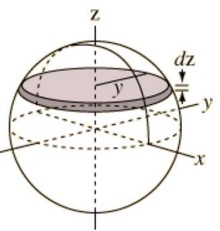
\includegraphics[width=5cm]{images/moi_sphere.jpg}
\end{figure}

Using volume mass density:
\[ \rho = \frac{M}{V} = \dv{m}{V} \implies \dd{m} = \rho\dd{V} \]

Moment of inertia of one disk about $z$-axis:
\[ \dd{I} = \frac{1}{2}y^2\dd{m} = \frac{1}{2}y^2\rho\dd{V} = \frac{1}{2}y^2\rho\pi y^2\dd{z} \]

Hence moment of inertia of sphere about $z$-axis is given by
\[ I_{CM} = \int \dd{I} = \frac{1}{2}\rho\pi\int_{-R}^R y^4\dd{z} = \frac{1}{2}\rho\pi\int_{-R}^R (R^2-z^2)^2\dd{z} = \frac{8}{15}\rho\pi R^5 = \boxed{\frac{2}{5}MR^2} \]

\begin{remark}
Another method is to sum up spherical hollow shells.
\end{remark}
\end{solution}

\begin{exmp}{}{}
Moment of inertia of a hollow cylinder with inner radius $R_1$ and outer radius $R_2$ about the central axis.
\end{exmp}

\begin{figure}[H]
    \centering
    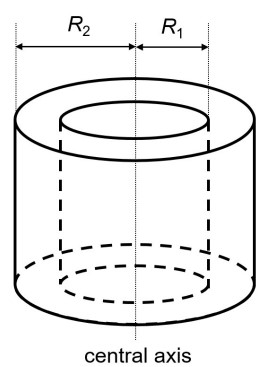
\includegraphics[width=5cm]{images/moi_hollow_cylinder.jpg}
\end{figure}

\begin{proof}
Consider a hollow cylindrical shell with radius $r$ and height $L$.

Using volume mass density,
\[ \rho=\dv{m}{V} \implies \dd{m}=\rho\dd{V} = 2\pi\rho Lr \dd{r} \]

Hence moment of inertia is 
\[ I = \int r^2\dd{m} = \int_{R_\text{in}}^{R_\text{out}} 2\pi\rho Lr^3 \dd{r} = \frac{\pi\rho L}{2}\sqbrac{r^4}_{R_\text{in}}^{R_\text{out}} = \boxed{\frac{1}{2}M(R_\text{out}^2+R_\text{in}^2)} \]
where $\rho = \dfrac{M}{\pi(R_\text{out}^2-R_\text{in}^2)L}$.
\end{proof}
\pagebreak

\begin{thrm}{Parallel axis theorem}{}
Moment of inertia $I$ about any axis parallel to axis through CM and a distance $D$ away is given by
\begin{equation}
I = I_{CM} + MD^2
\end{equation}
\end{thrm}

\begin{figure}[H]
    \centering
    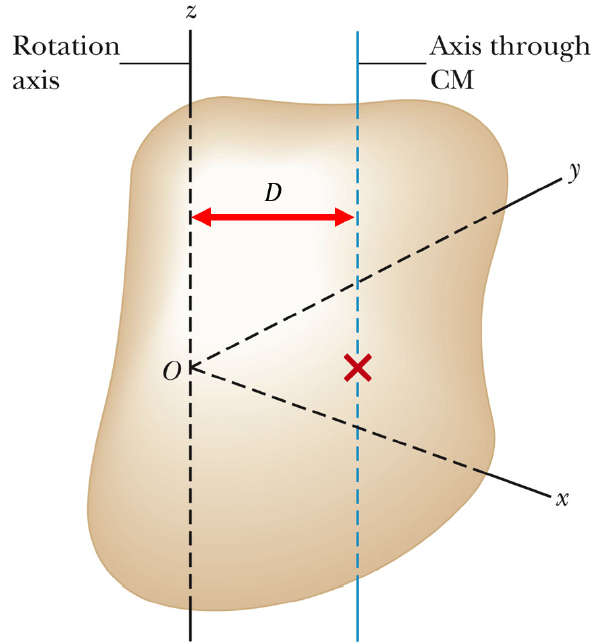
\includegraphics[width=7cm]{images/Parallel_axis_theorem.png}
    \caption{Parallel axis theorem}
\end{figure}

\begin{proof}
Moment of inertia about the $z$-axis is 
\[ I=\int r^2 \dd{m} = \int (x^2+y^2)\dd{m} \]
From the figure, $x=x^\prime+x_{CM}$ and $y=y^\prime+y_{CM}$ hence
\begin{align*}
I &= \int \left[(x^\prime+x_{CM})^2 + (y^\prime+y_{CM})^2\right] \dd{m} \\
&= \int (x^{\prime 2}+y^{\prime 2}) \dd{m} + ({x_{CM}}^2+{y_{CM}}^2) \int \dd{m} + 2x_{CM} \int x^\prime \dd{m} + 2y_{CM} \int y^\prime \dd{m}
\end{align*}
By definition of centre of mass, $\int x^\prime \dd{m} = \int y^\prime \dd{m} = 0$.

Given that $\int\dd{m}=M$ and $D^2={x_{CM}}^2+{y_{CM}}^2$,
\[ \boxed{I=I_CM+MD^2} \]
\end{proof}
\begin{figure}[H]
    \centering
    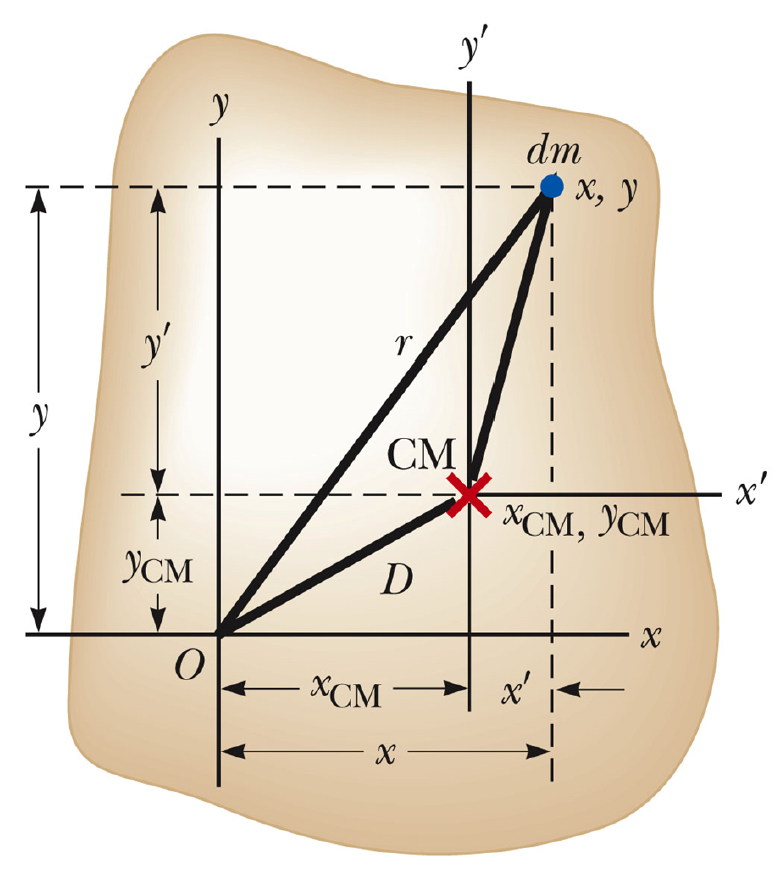
\includegraphics[width=7cm]{images/Parallel_axis_theorem2.png}
\end{figure}

\begin{exmp}{}{}
Consider a uniform rigid rod of mass $M$ and length $L$. Find the moment of inertia of the rod about an axis perpendicular to the rod through one end.
\end{exmp}

\begin{solution}
Moment of inertia is 
\[ \frac{1}{12}ML^2 + M\brac{\frac{L}{2}}^2 = \boxed{\frac{1}{3}ML^2} \]
\end{solution}

\begin{thrm}{Perpendicular axis theorem}{}
Sum of moments of inertia about any two perpendicular axes in the plane of the body is equal to the moment of inertia about an axis through the point of intersection, perpendicular to the plane of the object.
\begin{equation}
I_z = I_x + I_y
\end{equation}
This theorem works only for planar figures (2D bodies), i.e. bodies of negligible thickness.
\end{thrm}

\begin{proof}
\begin{align*}
I_z &= \int r^2 \dd{m} \\
&= \int (x^2+y^2) \dd{m} \\
&= \int x^2 \dd{m} + \int y^2 \dd{m} \\
\end{align*}
\end{proof}
\pagebreak

\subsection{Rotational kinetic energy}
We treat a rigid object as a collection of particles rotating about a fixed $z$-axis with an angular speed $\omega$.

Kinetic energy of the $i$-th particle is given by 
\[ K_i = \frac{1}{2} m_i {v_i}^2 = \frac{1}{2} m_i (r_i \omega)^2 = \frac{1}{2} m_i {r_i}^2 \omega^2 \]

Hence rotational kinetic energy possessed by a rigid object is given by 
\[ K = \sum_i K_i = \frac{1}{2}\left( \sum_i m_i {r_i}^2 \right) \omega^2 \]
\begin{equation}
K = \frac{1}{2} I \omega^2
\end{equation}

\begin{remark}
Notice the similarities between this and the formula for translational kinetic energy $K=\frac{1}{2}mv^2$.
\end{remark}
\pagebreak

\subsection{Torque}
\begin{defn}{Torque}{}
The measure of tendency of a force to \emph{rotate} an object about some axis.
\end{defn}

\begin{equation}
|\vb{\tau}| = F\ell = F\cdot r\sin\theta
\end{equation}
where $\ell = r\sin\theta$ is the \textbf{level arm}, i.e. the perpendicular distance from axis of rotation to the line of action of force.

Representing torque as a vector,
\begin{equation}
\mathbf{\tau} = \vb{r} \times \vb{F}
\end{equation}

\subsubsection{Torque and angular acceleration}
\begin{equation}
\vb{\tau} = I\alpha
\end{equation}
\begin{proof}
Consider a force $\dd{\vb{F}}_t$ acting on a mass element $\dd{m}$ of an extended object. 

From Newton's 2nd law,
\[ \dd{\vb{F}}_t = (\dd{m})a_t \implies d\vb{\tau} = r\dd{\vb{F}}_t = ra_t\dd{m} \]
Since $a_t=r\alpha$,
\[ \dd{\vb{\tau}} =  \alpha r^2\dd{m} \]
Net torque about origin due to all external forces is 
\[ \sum\vb{\tau} = \int\dd{\vb{\tau}} = \int\alpha r^2\dd{m} = \alpha\int r^2\dd{m} = \boxed{I\alpha}  \]
\end{proof}
\pagebreak

\subsection{Work, Energy, Power}
The work done by force $F$ on an object as it rotates through an infinitesimal distance $\dd{s}=r\dd{\theta}$ is
\[ \dd{W} = F\dd{s} = (F\sin\phi)r\dd{\theta} = \tau\dd{\theta} \]
Integrating both sides gives
\begin{equation}
W = \int \vb{\tau} \dd{\theta}
\end{equation}

Rate at which work is done by $F$ as the object rotates about the fixed axis through an angle $\dd{\theta}$ in a time interval $\dd{t}$ is
\[ \odv{W}{t} = \tau\odv{\theta}{t} \]
Hence power is
\begin{equation}
P=\tau\omega
\end{equation}

\begin{thrm}{Work--kinetic energy theorem}{}
Net work done by external forces in rotating a rigid body about a fixed axis equals the change in the object's rotational kinetic energy.
\begin{equation}
\sum W = \frac{1}{2}I\omega_f^2 - \frac{1}{2}I\omega_i^2
\end{equation}
\end{thrm}
\pagebreak

\subsection{Rolling motion}
In pure rolling motion, an object rolls without slipping. 

The object rotates through an angle $\theta$, so centre of mass moves a linear distance $s=R\theta$. 

Linear speed of centre of mass:
\begin{equation}
v_{CM} = R\omega
\end{equation}
\begin{derivation}
\[ v_{CM} = \odv{s}{t} = R\odv{\theta}{t} = R\omega \]
\end{derivation}

Linear acceleration of centre of mass:
\begin{equation}
a_{CM} = R\alpha
\end{equation}
\begin{derivation}
\[ a_{CM} = \odv{v_{CM}}{t} = R\odv{\omega}{t} = R\alpha \]
\end{derivation}

\textbf{Pure rolling motion} is a combination of 
\begin{itemize}
\item pure \textbf{translational motion} of centre of mass
\item pure \textbf{rotational motion} around centre of mass
\end{itemize}

Total kinetic energy of a rolling object is the \textbf{sum} of rotational kinetic energy about centre of mass and translational kinetic energy of centre of mass.
\begin{equation}
K = \frac{1}{2}I_{CM}\omega^2 + \frac{1}{2}M{v_{CM}}^2
\end{equation}
\begin{derivation}
Object rotates about point $P$, the point of contact with ground.

Total kinetic energy can be expressed as
\[ K=\frac{1}{2}I_P\omega^2 \]
where $I_P$ is the moment of inertia about an axis through $P$.

Using parallel axis theorem,
\[ I_P = I_{CM} + MR^2 \]

Hence 
\[ K = \frac{1}{2}I_{CM}\omega^2 + \frac{1}{2}M(R\omega)^2 = \boxed{\frac{1}{2}I_{CM}\omega^2 + \frac{1}{2}Mv_{CM}^2} \]
\end{derivation}
\pagebreak

\subsection{Angular momentum}
\begin{defn}{Angular momentum}{}
Cross product of instantaneous position vector $\vb{r}$ and linear momentum $\vb{p}$.
\begin{equation}
L \equiv \vb{r} \times \vb{p}
\end{equation}
\end{defn}

\begin{derivation}
From the definition of torque, $\vb{\tau} \equiv \vb{r}\times\vb{F}$,
\[ \sum\vb{\tau} = \vb{r}\times\sum\vb{F} = \vb{r}\times\odv{\vb{p}}{t} \]
Add the term $\odv{\vb{r}}{t}\times\vb{p}$ to the right-hand side, which is zero because $\odv{\vb{r}}{t}=\vb{v}$ which is parallel to $\vb{p}$.
\[ \sum\vb{\tau} = \vb{r}\times\odv{\vb{p}}{t} + \dv{\vb{r}}{t}\times\vb{p} = \dv{(\vb{r}\times\vb{p})}{t} = \boxed{\dv{\vb{L}}{t}} \]
\end{derivation}

Hence the torque acting on a particle is equal to the time rate of change of angular momentum.
\begin{equation}
\sum\mathbf{\tau} = \dv{\vb{L}}{t}
\end{equation}
This is the rotational analog of Newton's 2nd law.

\subsubsection{System of particles}
Total angular momentum of a system of particles about some point is defined as the vector sum of angular momentum of the individual particles.
\[ L_{total} = \sum_i L_i \]
Hence
\[ \sum_i \tau_i = \sum_i \odv{L_i}{t} = \odv{L_{total}}{t} \]

The torque acting on the particles of the system are due to internal forces between particles and external forces. However, net torque due to internal forces is zero as a result of Newton's 3rd law. Hence total angular momentum of system varies only if net external torque acts on the system:
\begin{equation}
\sum\mathbf{\tau}_\text{ext} = \dv{\vb{L}}{t}
\end{equation}

Net torque about axis through origin equals time rate of change of total angular momentum of system about that origin.

\begin{thrm}{}{}
Resultant torque acting on a system about axis through \underline{centre of mass} equals time rate of change of angular momentum \underline{regardless of motion of centre of mass}.
\end{thrm}

\subsubsection{Rigid body}
Angular momentum of one particle is
\begin{equation}
L \equiv mr^2\omega = mrv
\end{equation}

Taking the sum of angular momentum over all particles on a rigid body,
\[ \vb{L} = \sum_i \vb{L}_i = \brac{\sum_i m_i{r_i}^2}\omega = I\omega \]
\begin{equation}
L = I\omega
\end{equation}

Taking time derivative,
\[ \odv{L}{t} = I\odv{\omega}{t} = I\alpha \]
Hence
\begin{equation}
\sum\tau_{ext} = I\alpha
\end{equation}

\subsubsection{Conservation of angular momentum}
\begin{thrm}{}{}
Total angular momentum of a system is constant in both magnitude and direction if the resultant external torque acting on the system is zero.
\begin{equation}
\sum\tau_{ext} = \odv{L_{total}}{t} = 0
\end{equation}
\[ L_i = L_f \]
\end{thrm}
\pagebreak

\begin{exmp}{}{}
A uniform disc of radius $R$ is spinning about the vertical axis and placed on a horizontal surface. If the initial angular speed is $\omega$ and the coefficient of friction is $\mu$, determine the time before which the disc comes to rest.
\end{exmp}

\begin{solution}
A common mistake is to directly apply the equation $\tau=f_k\times R$ because the radius is not the same for all points on the disc.

Instead, we analyse using a ring of mass $\dd{m}$, radius $r$ and width $\dd{r}$, where all points on the ring have the same radius from the centre.

Torque of ring is
\[ \dd{\tau} = r \dd{f_k} = r(\mu_k g \dd{m}) = \mu_k g r \dd{m} \]

Torque of disk is
\[ \tau = \int \dd{\tau} = \int \mu_k g r \dd{m} = \mu_k g \int r \dd{m} \]

Using \textbf{area density}, 
\[ \sigma = \frac{M}{A} = \frac{\dd{m}}{\dd{A}}, \]
hence
\[ \frac{\dd{m}}{2\pi r}=\frac{M}{\pi R^2} \implies \dd{m} = \frac{M}{\pi R^2}2\pi r \]

Substituting this gives us 
\[ \tau = \mu_k g \int r \frac{M}{\pi R^2}2\pi r \dd{r} = \frac{2\mu_kMg}{R^2}\int_0^R r^2 \dd{r} = \frac{2\mu_kMg}{R^2} \frac{R^3}{3} = \boxed{\frac{2}{3}\mu_kMgR} \]

Using Newton's 2nd Law,
\[ \tau = I\alpha \implies \frac{2}{3}\mu_kMgR = \brac{\frac{1}{2}MR^2}\alpha \implies \alpha = \frac{4}{3}\frac{\mu_kg}{R} \]

Using angular acceleration, calculate the time taken:
\begin{align*}
\omega_f &= \omega_i-\alpha t \\
0 &= \omega - \alpha t \\
t &= \frac{\omega}{\alpha} \\
\Aboxed{t &= \frac{3}{4}\frac{R\omega}{\mu_kg}}
\end{align*}
\end{solution}
\pagebreak

\begin{exmp}{}{}
A uniform rod of mass $M$ and length $L$ is placed vertically with one end pinned to a frictionless horizontal floor. It starts to fall when it is given a small displacement. When the rod makes an angle $\theta$ with the vertical, find
\begin{enumerate}[label=(\alph*)]
\item the radial acceleration of the top of the rod;
\item the tangential acceleration of the top of the rod.
\end{enumerate}
\end{exmp}

\begin{solution}
Let $\tau_O$ denote torque about pin at point $O$. 

Using Newton's 2nd Law,
\[ \tau_O = I\alpha \implies Mg\brac{\frac{L}{2}\sin\theta} = \sqbrac{\frac{1}{12}ML^2+M\brac{\frac{L}{2}}^2}\alpha \implies \alpha = \frac{3}{2}\frac{g\sin\theta}{L} \]

Note that since the axis of rotation through the pin at $O$ is parallel to the axis through centre of mass, we use the \emph{parallel axis theorem} to determine $I$.

Using this value of angular acceleration, we can calculate tangential acceleration.
\[ a_t = L\alpha = \boxed{\frac{3}{2}g\sin\theta} \]

To calculate radial acceleration, recall that 
\[ a_r = \frac{{v_t}^2}{L} = L\omega^2 \]
To find $\omega$, recall that angular acceleration is the derivative of angular velocity with respect to time.
\begin{align*}
\odv{\omega}{t} &= \frac{3}{2}\frac{g\sin\theta}{L} \\
\odv{\omega}{\theta}\odv{\theta}{t} &= \frac{3}{2}\frac{g\sin\theta}{L}\\
\omega \dd{x} &= \frac{3}{2}\frac{g\sin\theta}{L}\dd{\theta} \\
\int_0^{\omega}\omega \dd{\omega} &= \int_0^{\theta}\frac{3}{2}\frac{g\sin\theta}{L}\dd{\theta} \\
\frac{\omega^2}{2} &= \frac{3g}{2L}(-\cos\theta+1)\\
\omega^2 &= \frac{3g}{L}(1-\cos\theta)
\end{align*}
Substituting this value of angular velocity gives us 
\[ \boxed{a_r=3g(1-\cos\theta)} \]
\end{solution}

\chapter{Celestial mechanics}
\section{Kepler's Laws}
Kepler's Laws are used to describe planetary motion.
\begin{thrm}{Kepler's 1st Law}{}
The orbit of every planet is an ellipse with the Sun at one of the two foci.
\end{thrm}

\begin{proof}
Kepler's 1st law indicates that the circular orbit is a very special case and elliptical orbits are the general situation.

\begin{figure}[H]
    \centering
    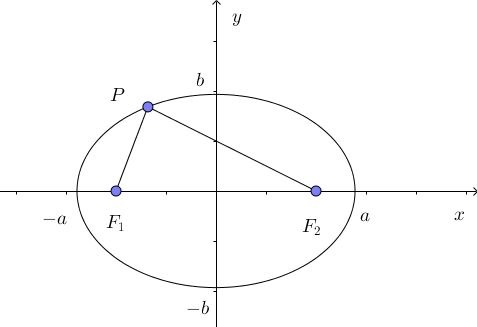
\includegraphics[width=10cm]{images/ellipse.jpg}
\end{figure}

An ellipse is mathematically defined by choosing two points $F_1$ and $F_2$, each of which is called a focus, and then drawing a curve through points for which $PF_1+PF_2$ is constant. 

The major axis is the longest distance through the centre between points on the ellipse. Semi-major axis is the distance $a$. The minor axis is the shortest distance. Semi-minor axis is the distance $b$. Eithr focus of the ellipse is located at a distance $c$ from the centre of ellipse, where $a^2=b^2+c^2$.

The eccentricity of an ellipse is defined as $e=\dfrac{c}{a}$, which describes the general shape of the ellipse. For a circle, $c=0$. Higher values of eccentricity correspond to longer and thinner ellipses. The range of values of the eccentricity for an ellipse is $0<e<1$.

\textbf{Aphelion}: point where the planet is the farthest away from the Sun (for object in orbit around Earth, this point is called the \textbf{apogee}), distance = $a+c$

\textbf{Perihelion}: point where the planet is the nearest to the Sun (for object in orbit around Earth, this point is called the \textbf{perigee}), distance = $a-c$
\end{proof}
\pagebreak

\begin{thrm}{Kepler's 2nd Law}{}
A line joining a planet and the Sun sweeps out equal areas during equal intervals of time.
\end{thrm}

\begin{proof}
Kepler's 2nd law is a consequence of the conservation of angular momentum.

By the law of conservation of angular momentum, 
\[ L = rp = mr^2\omega = mr^2\odv{\theta}{t} \]

Area of a small sector $\dd{A}$ swept out by the radial line is given by 
\[ \dd{A} = \frac{1}{2}r^2\dd{\theta} = \frac{1}{2}r^2\odv{\theta}{t}\dd{t} = \frac{1}{2}\frac{L}{m}\dd{t} \implies A=\frac{1}{2}\frac{Lt}{m} \]
Hence for constant $t$, $A$ is constant.
\end{proof}
\pagebreak

\begin{thrm}{Kepler's 3rd Law}{}
The ratio of the square of a planet's period of revolution to the cube of the semi-major axis of its orbit around the Sun is a constant, and this constant is the same for all planets.
\begin{equation}
T^2 = \frac{4\pi^2}{GM}a^3
\end{equation}
where $a$ is the length of the semi-major axis.
\end{thrm}

\begin{proof}
In the case of a circular orbit, gravitational force provides centripetal force for orbit.
\[ mr\omega^2 = G \frac{mM}{r^2} \]
Then, expressing the angular velocity $\omega$ in terms of the orbital period $T$ and then rearranging, results in Kepler's Third Law:

\[ mr\brac{\frac{2\pi}{T}}^2 = G\frac{Mm}{r^2} \implies T^2 = \brac{\frac {4\pi^2}{GM}}r^3 \implies T^2\propto r^3 \]
\end{proof}
\pagebreak

\section{Gravitational potential energy of spherical shell}
Let us consider a uniform spherical shell of mass $M$. Its mass per unit area will be $\sigma = \frac{M}{4\pi R^2}$. Consider a strip of width $R\dd{\theta}$ and radius $R\sin\theta$. The whole shell is made up of such strips.

\begin{figure}[H]
    \centering
    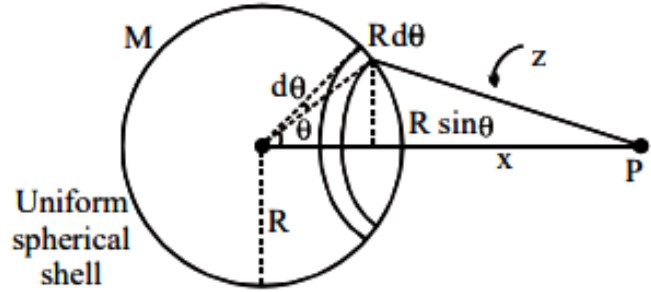
\includegraphics[width=8cm]{images/spherical_shell_gpe.jpg}
\end{figure}

Potential at $P$ due to the ring is given by
\[ \dd{V} = -G\frac{\dd{M}}{z} \] 
\begin{equation}\tag{1}
\dd{V} = -G\frac{2\pi R^2\sin\theta\dd{\theta}}{z}
\end{equation}

Now, 
\[ z = \sqrt{(x-R\cos\theta)^2 + (R\sin\theta)^2} \]
\[ z^2 = x^2 + R^2 - 2xR\cos\theta \]

Differentiating, we get
\[ 2xR\sin\theta=2z\dd{z} \]
\begin{equation}\tag{2}
\sin\theta\dd{\theta} = \frac{z\dd{z}}{xR}
\end{equation}

From (1) and (2),
\[ \dd{V} = -\frac{GM}{2z}\frac{z\dd{z}}{xR} = -\frac{GM}{2xR}\dd{z} \]

\textbf{Case 1: P lies outside the shell}

In this case $x-R \le z \le x-R$. Therefore potential is 
\[ V = -\frac{GM}{2xR}\int_{x-R}^{x+R}\dd{z} = -\frac{GM}{2xR}2R = -\frac{GM}{x} \]

\textbf{Case 2: P lies inside the shell}

In this case $R-x \le z \le x-R$. Therefore potential is 
\[ V=-\frac{GM}{2x}\int_{R-x}^{x+R}\dd{z}=-\frac{GM}{R} \]
\pagebreak

\section{Elliptical orbits and orbital transfers}
To solve problems involving orbital transfers, the key strategy is to work from energy considerations in satellite motion. Recall that the total mechanical energy $E$ of a bound satellite system is $E=-\frac{GMm}{2r}$.

A similar expression for $E$ for elliptical orbits is the same, with $r$ replaced by the semi-major axis of length $a$:
\[ E=-\frac{GMm}{2a} \]
\pagebreak

\section{Effective radial potential}
An orbiting satellite of mass $m$ under the influence of the gravitational field due to the Earth of mass $M$, is at a distance $r$ from the centre of Earth.

Assuming that the system consists of Earth and a satellite and the mass of Earth is many times larger than that of satellite, total energy $U$ of the system is given by 
\[ E_\text{total} = \frac{1}{2}mv_r^2 + \frac{L^2}{2mr^2} - \frac{GMm}{r} \]
where $L$ is angular momentum of satellite, $v_r$ is radial velocity of satellite.

\begin{derivation}
Total energy of a moving satellite m under the influence of the gravitational field due to the Earth of mass M is given by: 
\[ U = E_k+E_p = \frac{1}{2}mv^2 - \frac{GMm}{r} \]
Since the satellite has an ellipsoidal orbit,
\[ v^2 = v_t^2 + v_r^2 \]
Since satellite is in a central force field $\tau=\vb{r}\times\vb{F}=\mathbf{0}$ and $L=mrv_t$.

Therefore, sub into equations and simplifying, 
\[ E_\text{total} = \frac{1}{2}mv_t^2 + \frac{1}{2}mv_r^2 - \frac{GMm}{r} = \boxed{\frac{1}{2}mv_r^2 + \frac{L^2}{2mr^2} - \frac{GMm}{r}} \]
\end{derivation}

Hence \textbf{effective potential} is given by
\[ U_\text{eff} = E_\text{total} - \text{KE}_r = \boxed{\frac{L^2}{2mr^2} - \frac{GMm}{r}} \]

\begin{equation}
U_\text{eff} = \frac{L^2}{2mr^2} - \frac{GMm}{r}
\end{equation}

\chapter{Hydrodynamics}
\section{Fluid Statics}
\begin{thrm}{Pascal's principle}{}
In equilibrium, the pressure in a static varies with height:
\begin{equation}
\dv{P}{y}=-\rho g
\end{equation}

This always holds in equilibrium. For instance, if we squeeze a sealed container of fluid, increasing the pressure locally, then this pressure increase must propagate throughout the entire fluid to maintain $dP/dy = -\rho g$.
\end{thrm}

\begin{thrm}{Archimedes' Principle}{}
An object in a fluid experiences an upward buoyant force due to the different pressures on its top and bottom sides. The force is equal in magnitude to the weight of the fluid displaced.
\end{thrm}

\subsection{Surface tension}
Surface tension and the associated energy, capillary pressure.
\pagebreak

\section{Fluid Mechanics}
Steady flow is where every fluid particle arriving at a given point has the same velocity.

Viscosity is the degree of internal friction; resistance that 2 adjacent layers of the fluid have to move relative to each other.

Ideal fluid flow:
\begin{enumerate}
    \item Non-viscous
    \item Steady
    \item Incompressible
    \item Irrotational
\end{enumerate}

\begin{thrm}{Equation of continuity}{}
This equation says that the flow of fluid through a tube of changing cross section is constant.
\begin{equation}
A_1 v_1 = A_2 v_2
\end{equation}
\end{thrm}

\begin{derivation}
Conservation of mass

Consider the case of a fluid moving from a region of cross-sectional area $A_1$ to a region of area $A_2$. Since the fluid is incompressible, the same amount of it leaves each region and enters the other region during the same time interval.

Volume of fluid that flows into the tube across $A_1$ in time interval $\Delta t$ is \[ \Delta V_1=A_1v_1\Delta t \] 
Hence the mass of fluid that flows into the tube in time $\Delta t$ is
\[ \Delta m_1 = \rho\Delta V_1 = \rho A_1v_1\Delta t \]
Similarly, the mass of fluid that flows across $A_2$ is
\[ \Delta m_2 = \rho\Delta V_2 = \rho A_2v_2\Delta t \]
Equating the two masses,
\[ \Delta m_1 = \Delta m_2 \implies \boxed{A_1v_1=A_2v_2} \]
\end{derivation}

\begin{thrm}{Bernoulli's equation}{}
\begin{equation}
P_1 + \frac{1}{2}\rho {v_1}^2 + \rho gy_1 = P_2 + \frac{1}{2}\rho {v_2}^2 + \rho gy_2 = \text{constant}
\end{equation}
\end{thrm}

\begin{derivation}
Conservation of energy

% https://www.khanacademy.org/science/physics/fluids/fluid-dynamics/a/what-is-bernoullis-equation
\end{derivation}

\subsection{Viscosity}


\begin{thrm}{Poiseuille's Law}{}
\begin{equation}
P_1 - P_2 = 8\frac{Q\eta L}{\pi R^4}
\end{equation}
where $Q$ is the flow rate, $\eta$ is the coefficient of viscosity.
\end{thrm}


\part{Oscillations and Waves}
\chapter{Single oscillator}
\section{Harmonic oscillation}
\vocab{Restoring force or torque} is the resultant force or torque directed towards the equilibrium position.

\vocab{Simple harmonic motion}: restoring force or torque is linear, i.e. net force is directed towards the equilibrium position and is proportional to displacement from equilibrium.

\subsection{Kinematics and Energy}
Frequency and period are related by
\begin{equation}
f=\frac{1}{T}
\end{equation}

Angular frequency, frequency and period are related by
\begin{equation}
\omega = 2\pi f = \frac{2\pi}{T}
\end{equation}

\textbf{Displacement}:
\begin{equation}
{x(t)=A\cos\brac{\omega t+\phi_0}
}\end{equation}
where $A$ and $\phi_0$ are constants determined by initial conditions $x$ ($t=0$) and $v_x$ ($t=0$).
\begin{proof}[Derivation]
By Newton's 2nd Law,
\[ F_x=-kx_x=ma_x \implies a_x=-\frac{k}{m}x \implies \dv[2]{x(t)}{t}=-\frac{k}{m}x(t)=-\omega^2x(t) \]
which is a second-order ordinary differential equation.
\end{proof}

\textbf{Velocity}:
\begin{equation}
{v_x(t)=\dv{x(t)}{t}=-\omega A\sin(\omega t+\phi_0)
}\end{equation}

\textbf{Acceleration}:
\begin{equation}
{a_x(t)=\dv{v_x(t)}{t}=-\omega^2 A\cos(\omega t+\phi_0)
}\end{equation}

\textbf{Kinetic energy}:
\begin{equation}
{K(t)=\frac{1}{2}mv_x(t)^2=\frac{1}{2}m\omega^2A^2\sin^2\brac{\omega t+\phi_0}
}\end{equation}

\textbf{Potential energy}:
\begin{equation}
{U(t)=\frac{1}{2}kx(t)^2=\frac{1}{2}kA^2\cos^2\brac{\omega t+\phi_0}
}\end{equation}

Total energy is the sum of KE and PE:
\begin{equation}
{E(t)=K(t)+U(t)=\frac{1}{2}kA^2
}\end{equation}

\subsection{Newton’s Approach}
Consider a spring-mass system, as shown below:
\begin{figure}[H]
    \centering
    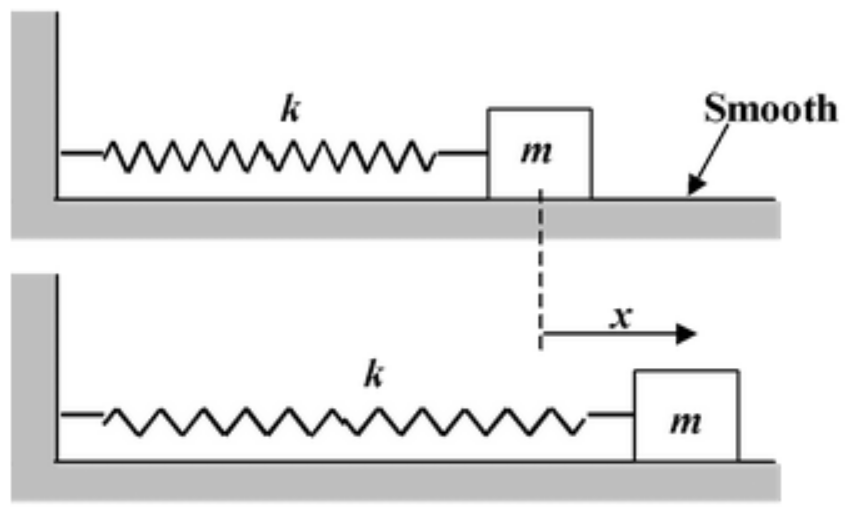
\includegraphics[width=8cm]{images/spring_mass_system.png}
\end{figure}

By Newton's 2nd Law, 
\begin{align*}
\sum\vb{F}(t) &= m\vb{a}(t) \\
-kx(t) &= m\dv[2]{x(t)}{t} \\
\dv[2]{x(t)}{t} &= -\frac{k}{m}x(t)
\end{align*}
where $\dfrac{k}{m}$ is a constant.

We define
\[ \omega^2 \equiv \frac{k}{m} \]

Then \[ \dv[2]{x(t)}{t} = -\omega^2x(t) \]

This 2nd order differential equation has the general solution for the \textbf{displacement function}:
\[ x(t)=A\cos\omega t + B\sin\omega t \]
where constants $A$ and $B$ are determined by the initial conditions, such as $x(0)=0$, $v(0)=v_0$. This gives us $A=x_0$ and $B=\frac{v_0}{\omega}$. 

Hence we have the displacement function for a particular oscillation:
\[ \boxed{x(t)=x_0\cos\omega t + \frac{v_0}{\omega}\sin\omega t} \]

Considering the period $T$, since the displacement function is periodic, we have $x(t)=x(t+T)$. Plugging this into the displacement function above, we have 
\begin{align*}
\cos(\omega t) &= \cos(\omega t+\omega T) \\
\cos(\omega t) &= \cos(\omega t+\omega T)
\end{align*}
The property of the sine and cosine functions gives us \[ \omega T=2\pi \implies \omega=\frac{2\pi}{T} \text{ and } \omega=2\pi f \]

This gives us \[ T=2\pi\sqrt{\frac{m}{k}} \]
\pagebreak

Using \textbf{simple pendulum motion} as another example, 

\begin{figure}[H]
    \centering
    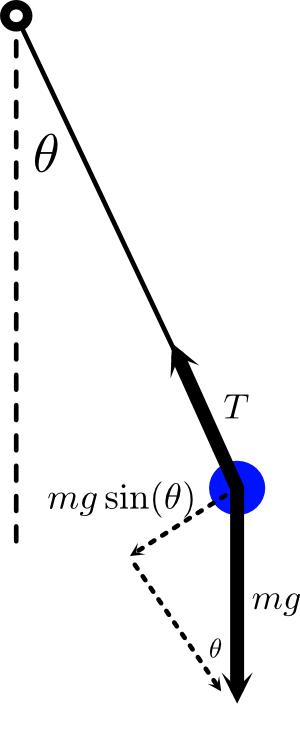
\includegraphics[width=4cm]{images/pendulum-fbd.png}
\end{figure}

By Newton's 2nd Law, 
\[ \vb{F}_t=m\vb{a}_t \implies -mg\sin\theta(t)=m\dv[2]{s(t)}{t} \]
By small angle approximation, $\sin\theta \approx \theta$.
\[ \dv[2]{\theta(t)}{t} = -\frac{g}{L}\sin\theta(t) \implies \dv[2]{\theta(t)}{t} \approx \frac{g}{L}\sin\theta(t) \equiv -\omega^2\theta(t) \]
Period of the motion:
\[ T=\frac{2\pi}{\omega}=2\pi\sqrt{\frac{L}{g}} \]
\pagebreak

For the \textbf{physical pendulum motion}, an \textbf{extended object} swings back and forth on a pivot under the influence of gravity.

\begin{figure}[H]
    \centering
    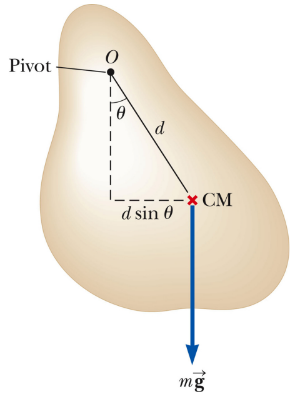
\includegraphics[width=6cm]{images/physical_pendulum.png}
\end{figure}

Net torque with respect to the pivot, using $\tau = I\alpha$:
\[ -mgd\sin\theta(t)=I\dv[2]{\theta(t)}{t} \implies \dv[2]{\theta(t)}{t}=-\frac{mgd}{I}\sin\theta(t) \]
By small approximation, $\sin\theta \approx \theta$
\[ \dv[2]{\theta(t)}{t} = -\frac{mgd}{I}\theta(t) \equiv -\omega^2\theta(t) \]
Hence period of the motion is given by
\[ T=\frac{2\pi}{\omega}=2\pi\sqrt{\frac{I}{mgd}} \]

\subsection{Energy conservation}
Using the above example of the simple pendulum motion, we analyse the energy of the pendulum.
\begin{align*}
E(t) &= \text{Rotational KE} + \text{GPE} \\
&= \frac{1}{2}I\omega^2 + mgL(1-\cos\theta(t)) \\
&= \frac{1}{2}(mL^2)\sqbrac{\dv{\theta(t)}{t}}^2 + mgL(1-\cos\theta(t)) \\
\dv{E(t)}{t} &= mL^2\dv{\theta(t)}{t}\dv[2]{\theta(t)}{t} + mgL\sin\theta(t)\dv{\theta(t)}{t}
\end{align*}

Since energy is conserved, total energy remains constant, hence
\[ \dv{E(t)}{t}=0 \implies L\dv[2]{\theta}{t} + g\sin\theta(t) = 0 \implies \dv[2]{\theta}{t}=-\frac{g}{L}\sin\theta(t) \]
and the rest follows.
\pagebreak

\begin{exmp}
A mass $M$ is connected to two springs 1, 2 of spring constants $k_1$ and $k_2$ and slides on a smooth horizontal table. In the equilibrium position it is given a velocity $v_0$ towards spring 2.
\begin{enumerate}[label=(\alph*)]
\item Find the period of the motion.
\item Find the amplitude of the motion.
\end{enumerate}
\end{exmp}

\begin{figure}[H]
    \centering
    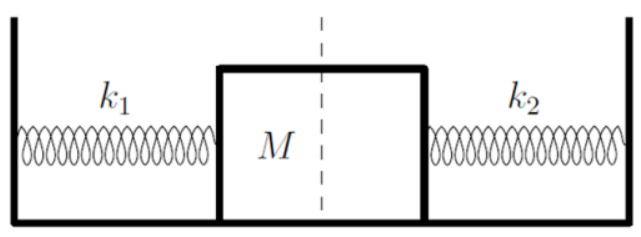
\includegraphics[width=6cm]{images/two_springs.png}
\end{figure}

\begin{proof}[Solution]
By Newton's 2nd Law,
\[ \sum\vb{F}(t)=-(k_1+k_2)x(t) \implies \dv[2]{x}{t}=-\frac{k_1+k_2}{M}x \implies \omega^2\equiv\frac{k_1+k_2}{M} \]
Period:
\[ \boxed{T=\frac{2\pi}{\omega}=2\pi\sqrt{\frac{M}{k_1+k_2}}} \]

By conservation of energy, loss in kinetic energy is converted to gain in elastic potential energy.
\[ \frac{1}{2}m{v_0}^2 = \frac{1}{2}k_1{x_0}^2 + \frac{1}{2}k_2{x_0}^2 \implies \boxed{x_0 = \sqrt{\frac{m{v_0}^2}{k_1+k_2}}} \]
\end{proof}
\pagebreak

\section{Damped oscillations}
Exponential decay of damped oscillations

\section{Forced oscillations and resonance}
resonance of sinusoidally forced oscillators: amplitude and phase shift of steady state oscillations. 

Free oscillations of LC-circuits; mechano-electrical analogy; positive feedback as a source of instability; generation of sine waves by feedback in a LC-resonator.


\chapter{Waves}
\section{Basics}
Propagation of harmonic waves: phase as a linear function of space and time; wave length, wave vector, phase and group velocities; exponential decay for waves propagating in dissipative media; transverse and longitudinal waves; the classical Doppler effect.

\section{Waves in inhomogeneous media}
Fermat’s principle, Snell’s law.

\section{Sound waves}
speed as a function of pressure (Young’s or bulk modulus) and density, Mach cone.

\section{Energy}
Energy carried by waves: proportionality to the square of the amplitude, continuity of the energy flux.
\pagebreak

\chapter{Interference and diffraction}
\section{Interference}
Superposition of waves: coherence, beats, standing waves, Huygens’ principle, interference due to thin films (conditions for intensity minima and maxima only).

\section{Diffraction}
Diffraction from one and two slits, diffraction grating, Bragg reflection.
\pagebreak

\chapter{Interaction of electromagnetic waves with matter}
Dependence of electric permittivity on frequency (qual-
itatively); refractive index; dispersion and dissipation of
electromagnetic waves in transparent and opaque ma-
terials. Linear polarisation; Brewster angle; polarisers;
Malus’ law.
\pagebreak

\chapter{Light and Optics}
\section{}

Approximation of geometrical optics: rays and optical images; a partial shadow and full shadow. 
Thin lens approximation; construction of images created by ideal thin lenses; thin lens equation.
Luminous flux and its continuity; illuminance; luminous intensity.
\pagebreak

\chapter{Optical devices}
Telescopes and microscopes: magnification and resolv-
ing power; diffraction grating and its resolving power;
interferometers.

\chapter{Relativity}
Principle of relativity and Lorentz transformations for
the time and spatial coordinate, and for the energy and
momentum; mass-energy equivalence; invariance of the
spacetime interval and of the rest mass. Addition of par-
allel velocities; time dilation; length contraction; relativ-
ity of simultaneity; energy and momentum of photons
and relativistic Doppler effect; relativistic equation of
motion; conservation of energy and momentum for elas-
tic and non-elastic interaction of particles.




% https://web.njit.edu/~vitaly/121/notes121.pdf
\part{Electromagnetic Fields}
\chapter{Electric Fields}
\section{Direct-Current Circuits}
\subsection{Electric Current and Resistance}
\subsubsection{Current}
The unit of current is defined in terms of the attractive force between two currents flowing in a parallel direction. Suppose the attractive force acting between two identical straight, parallel currents located one meter apart from each other is $2 \times 10^{-7}$ N for every meter of wire. Then, we define the amount of this current to be 1 A (ampere). 

An electric current of 1 A carries an electric charge of 1 C (coulomb) in 1 s. 

\subsubsection{Potential difference}
When the energy needed to carry an electric charge of 1 C against a potential difference (also called voltage) is 1 J (joule), this potential difference is defined to have a value of 1 V (volt).

\subsubsection{Resistance}
 When a voltage of 1 V is applied to a conductor, and a current
of 1 A flows in the conductor, the electric resistance of the conductor is defined to have a value of 1 $\Sigma$ (ohm).

The resistance of a conductor $R$ is defined in terms of the voltage applied to the conductor $V$ and the current flowing in the conductor $I$ as $R \equiv \dfrac{V}{I}$. This relation can be expressed as
\begin{equation}
{V=IR
}\end{equation}

\subsubsection{Ohm's Law}
\begin{thrm}{Ohm's Law}{}
When the resistance of the conductor $R$ is independent of the applied voltage $V$ or current $I$, the conductor satisfies \textbf{Ohm’s law}.

Such a resistance is called an \textbf{ohmic resistance}. The resistance of some conductors varies with voltage or current, and such a resistance is called a non-ohmic resistance.
\end{thrm}

\subsubsection{Resistivity}
The resistance of a conductor $R$ is proportional to its length $l$ and
inversely proportional to its cross-sectional area $A$:
\begin{equation}
{R = \rho \frac{l}{A}
}\end{equation}

where $\rho$ is the resistivity of the conductor, the value of which depends on the material and its temperature.

\subsection{Kirchhoff’s Rules}
\begin{thrm}{Kirchhoff ’s junction rule}{}
At any junction in an electric circuit, sum of the currents flowing into and out of that junction are equal.
\begin{equation}
\sum I_\text{in} = \sum I_\text{out}
\end{equation}
\end{thrm}

\begin{proof}
This rule implies the conservation of charge.
\end{proof}

The influence that makes a current flow from a lower to a higher potential is called an electromotive force (emf).

\begin{thrm}{Kirchhoff’s loop rule}{}
In any closed loop of an electric circuit, sum of all the electric potential differences around a loop is zero.
\[ \sum \Delta V = 0 \]
\end{thrm}
\pagebreak

\section{Electrostatics}
\subsection{Charge}
Charge carriers are protons and electrons, where protons have a positive charge $+e$ and electrons have a negative charge $-e$.

$e$ is the fundamental charge, $e=1.60\times10^{-19}$ \unit{C}.

Charge is quantised; it comes in discrete quantities in intervals of the fundamental charge.
\[ Q=ne \]
where $n$ is an integer number of excess positive or negative charges on the object.

\subsection{Electric force and field}
In an \textbf{electric field}, an \textbf{electric force} is exerted on a charged object placed in the field.

\begin{figure}[H]
    \centering
    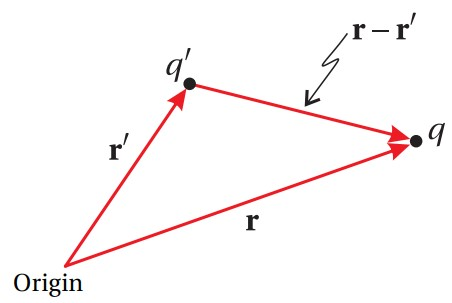
\includegraphics[width=7cm]{images/coulomb_law.jpg}
\end{figure}

The force on a point charge $q$ located at $\vb{r}$ exerted by another point charge $\vb{q}^\prime$ located at $\vb{r}^\prime$ is
\begin{equation}
{\vb{F} = q\vb{E}(\vb{r})
}\end{equation}
where
\begin{equation}
{\vb{E}(\vb{r}) = \frac{q^\prime}{4\pi\varepsilon_0} \frac{\vb{r}-\vb{r}^\prime}{|\vb{r}-\vb{r}^\prime|^3}
}\end{equation}
This relationship is known as \textbf{Coulomb’s law}. The force is directed along the vector $\vb{r}-\vb{r}^\prime$, which points from charge $q^\prime$ to $q$. 
The familiar inverse square law can be seen by noting that $\dfrac{\vb{r}-\vb{r}^\prime}{|\vb{r}-\vb{r}^\prime|}$ is a unit vector.

\begin{thrm}{Coulomb's law}{}
Consider the electric field produced by a point charge in vacuum. When a point test charge $q$ is located at a distance $r$ from a point source charge $Q$, the electric force that two charges $q$ and $Q$ exert on each other is
\begin{equation}
{\vb{F} = \frac{Qq}{r^2}
}\end{equation}
where $\varepsilon_0$ is the permittivity of vacuum.
\end{thrm}

Dividing both sides of the above equation by $q$ gives us electric field strength $\vb{E}$:
\begin{equation}
{\vb{E} = \frac{1}{4\pi\varepsilon_0}\frac{Q}{r^2}
}\end{equation}

We use electric field lines to visualise an electric field. An electric field line is a curve or line whose tangent at point gives the direction of the electric field vector $\vb{E}$ at that point. The number of electric field lines through a unit area perpendicular to $\vb{E}$ is equal to the magnitude of $\vb{E}$. Electric field lines are directed away from positive to negative charges, never intersect one another, and are never created nor annihilated in vacuum.

\subsection{Electric potential and energy}
Electric force is a conservative force. Work done by electric force on charge $q$ when the charge moves from position A to position B does not depend on the path taken.

Since work done by electric force only depends on the location of the initial (A) and final (B) positions, we can define an electrical potential energy function $U(r)$ that depends on position $r$. Work done by electric force $F_E$ on a charge in going from position A (defined by position vector, $r_A$) to position B (defined by position vector $r_B$) can be written as:
\[ W = \int_A^B \vb{F}_E \cdot \dd{\vb{r}} = -\Delta U = -\sqbrac{U(r_B)-U(r_A)} \]
Work done by electric force when $q$ moves from A to B is given by
\[ W = \int_A^B F_E\cdot\dd{r} = \int_{r_A}^{r_B} k\frac{Qq}{r^2} \dd{r} = kQq \int_{r_A}^{r_B} \frac{1}{r^2} \dd{r} = kQq\sqbrac{-\frac{1}{r}}_{r_A}^{r_B} = -\brac{\frac{kQq}{r_B} - \frac{kQq}{r_A}} \]

Hence electric potential energy is
\begin{equation}
U = \frac{1}{4\pi\epsilon_0}\frac{Qq}{r}
\end{equation}

Electric potential is the electric potential energy per unit charge, given by
\begin{equation}
V=\frac{1}{4\pi\varepsilon_0}\frac{Q}{r}
\end{equation}

\subsection{Continuous charge distribution}
A system of charges can be modelled as a \textbf{continuous charge distribution} when the electric field strength or electric potential due to the system is to be computed at a point much further than the distance between charges within the system.

Electric field strength or electric potential due to a continuous charge distribution is evaluated for each \textbf{infinitesimally small charge element}.

Electric field strength at a point due to charge element $\dd{q}$:
\[ \dd{\vb{E}} = \frac{\dd{q}}{4\pi\varepsilon_0r^2}\hat{\vb{r}} \]

Electric potential due to $\dd{q}$:
\[ \dd{V} = \frac{\dd{q}}{4\pi\varepsilon_0r} \]

Hence total electric field strength due to continuous charge distribution is 
\begin{equation}
\vb{E} = \frac{1}{4\pi\varepsilon_0} \int \frac{\dd{q}}{r^2} \hat{\vb{r}}
\end{equation}

and total electric potential is
\begin{equation}
V = \frac{1}{4\pi\varepsilon_0} \int \frac{\dd{q}}{r}
\end{equation}

The concept of \textbf{charge density} can be utilised most of the time for uniform charge distribution:
\begin{itemize}
\item \textbf{Linear charge density} $\lambda$ (charge uniformly distributed along line):
\[ \lambda = \frac{Q}{L} \]
\item \textbf{Surface charge density} $\sigma$ (charge uniformly distributed on surface):
\[ \sigma = \frac{Q}{A} \]
\item \textbf{Volume charge density} $\rho$ (charge uniformly distributed on volume):
\[ \rho = \frac{Q}{V} \]
\end{itemize}

These can be summarised as
\begin{equation*}
\dd{q} = \begin{cases}
    \lambda\dd{A} & \text{linear distribution} \\
    \sigma\dd{A} & \text{surface (area) distribution} \\
    \rho\dd{V} & \text{volume distribution} \\
\end{cases}
\end{equation*}
\pagebreak

Electric Field on the Axis of a Rod:
\begin{exmp}
A rod of length $L$ has a uniform positive charge per unit length $\lambda$ and a total charge $Q$. 

Calculate the electric field strength and the electric potential at a point $P$ that is located along the long axis of the rod and is a distance $a$ from one end.
\end{exmp}

%\begin{figure}[H]
%\centering
%\begin{tikzpicture}
%    \draw[-to] (-3,0) -- (10,0) \node [right] {$x$};
%    \draw[-to] (0,-3) -- (0,6) \node [above] {$y$};
%\end{tikzpicture}
%\end{figure}

\begin{proof}[Solution]
Set up coordinate system: rod lies on $x$-axis, point $P$ lies on origin at a distance $a$ from rod.

The electric field strength $\dd{\vb{E}}$ at $P$ due to charge element $\dd{q}$ is in the negative $x$ direction, since each charge element carries a positive charge.

Using linear charge density,
\[ \lambda = \frac{Q}{L} = \odv{q}{x} \implies \dd{q}=\lambda\dd{x} \]

Electric field strength at $P$ due to element $\dd{x}$ at a distance $x$ from $P$ is 
\[ \dd{\vb{E}} = \frac{\dd{q}}{4\pi\varepsilon_0x^2} = \frac{\lambda\dd{x}}{4\pi\varepsilon_0x^2} \]
Hence total electric field strength at $P$ is
\[ \vb{E} = \int \dd{\vb{E}} = \int_a^{L+a}\frac{\lambda\dd{x}}{4\pi\varepsilon_0x^2} = \boxed{\frac{Q}{4\pi\varepsilon_0a(L+a)}} \]

Similarly, electric potential at $P$ due to element $\dd{x}$ is 
\[ \dd{V} = \frac{\dd{q}}{4\pi\varepsilon_0x} = \frac{\lambda\dd{x}}{4\pi\varepsilon_0x} \]
Hence total electric potential at $P$ is
\[ V = \int \dd{V} = \int_a^{L+a} \frac{\lambda\dd{x}}{4\pi\varepsilon_0x} = \boxed{\frac{Q}{4\pi\varepsilon_0}\ln\brac{\frac{L+a}{a}}} \]

The answers can be verified by checking if $E=-\odv{V}{a}$ is valid.
\end{proof}
\pagebreak

Electric Field on the Axis of a Ring:
\begin{exmp}
A ring of radius $a$ carries a uniformly distributed positive total charge $Q$. 

Calculate electric field strength and electric potential at a point $P$ lying a distance $x$ from its centre along the central axis perpendicular to the plane of the ring.

Hence determine the positions where the magnitude of electric field strength is maximum.
\end{exmp}

\begin{proof}[Solution]
Electric field strength $\dd{\vb{E}}$ at $P$ due to charge element $\dd{q}$ can br resolved into components
\begin{itemize}
\item $\dd{\vb{E}}_x$ parallel to the axis of the ring
\item $\dd{\vb{E}}_y$ perpendicular to the axis.
\end{itemize}
For charge elements on opoisite sides of the ring, $\dd{\vb{E}}_y$ cancel out, so we only need to consider parallel components $\dd{\vb{E}}_x$.

Let $\theta$ be the angle between axis of ring and line joining $\dd{q}$ and $P$. Then
\[ \dd{\vb{E}}_x = \dd{\vb{E}}\cos\theta \]

Electric field strength at $P$ (at a distance $r$, perpendicular distance $x$ from ring) due to element $\dd{q}$ is
\[ \dd{\vb{E}} = \frac{\dd{q}}{4\pi\varepsilon_0r^2}\cos\theta = \frac{x\dd{q}}{4\pi\varepsilon_0(a^2+x^2)^\frac{3}{2}} \]
since $\cos\theta=\dfrac{x}{r}$ and $r=\sqrt{a^2+x^2}$.

Since all elements make the same contribution to the field at $P$ as they are all equidistant from this point, total electric field strength at $P$ is
\[ \vb{E} = \int \dd{\vb{E}} = \int \frac{x\dd{q}}{4\pi\varepsilon_0(a^2+x^2)^\frac{3}{2}} = \boxed{\frac{Qx}{4\pi\varepsilon_0(a^2+x^2)^\frac{3}{2}}} \]

Electric potential at $P$ due to element $\dd{q}$ is
\[ \dd{V} = \frac{\dd{q}}{4\pi\varepsilon_0r} = \frac{\dd{q}}{4\pi\varepsilon_0(a^2+x^2)^\frac{1}{2}} \]
Hence total electric potential at $P$ is
\[ V = \int\dd{V} = \int \frac{\dd{q}}{4\pi\varepsilon_0(a^2+x^2)^\frac{1}{2}} = \boxed{\frac{Q}{4\pi\varepsilon_0(a^2+x^2)^\frac{1}{2}}} \]

To evaluate position where $\vb{E}$ is maximum,
\[ \odv{\vb{E}}{x} = \frac{Q}{4\pi\epsilon_0}\sqbrac{\frac{a^2-2x^2}{(a^2+x^2)^\frac{5}{2}}} = 0 \implies \boxed{x=\pm\frac{a}{\sqrt{2}}} \]
\end{proof}
\pagebreak

Electric Field Due to a Uniformly Charged Disk:
\begin{exmp}
A disk of radius $R$ has a uniform surface charge density $\sigma$.

Calculate the electric field strength and electric potential at a point $P$ lying a distance $x$ from its centre along the central axis perpendicular to the disc.

Hence derive the electric field strength of an infinite, uniformly charged plate.
\end{exmp}

\begin{proof}[Solution]
A disk can be considered to be a set of concentric rings with diameter $r$ and thickness $\dd{r}$. Since surface charge density $\sigma=\frac{Q}{A}=\frac{dq}{dA}$, charge of one ring is
\[ \dd{q} = \sigma\dd{A} = \sigma\cdot2\pi\dd{r} \]
so the parallel electric field strength at $P$ due to this ring is 
\[ \dd{E} = \frac{x\dd{q}}{4\pi\varepsilon_0(r^2+x^2)^\frac{3}{2}} = \frac{\sigma rx\dd{r}}{2\varepsilon_0(r^2+x^2)^\frac{3}{2}} \]
Hence total electric field strength at $P$ is
\[ E = \int\dd{E} = \frac{\sigma x}{2\epsilon_0} \int_0^R\frac{r\dd{r}}{(r^2+x^2)^\frac{3}{2}} = \frac{\sigma x}{2\epsilon_0} \sqbrac{-\frac{1}{(r^2+x^2)^\frac{1}{2}}}_0^R = \boxed{\frac{\sigma}{2\varepsilon_0}\sqbrac{1-\frac{x}{(R^2+x^2)^\frac{1}{2}}}} \]

Similarly, electric potential at $P$ due to the ring is 
\[ \dd{V} = \frac{\sigma r\dd{r}}{2\varepsilon_0(r^2+x^2)^\frac{1}{2}} \]
Hence total electric potential at $P$ is
\[ V = \int\dd{V} = \frac{\sigma}{2\varepsilon_0}\int_0^R\frac{r\dd{r}}{(r^2+x^2)^\frac{1}{2}} = \frac{\sigma}{2\varepsilon_0}\sqbrac{(r^2+x^2)^\frac{1}{2}}_0^R = \boxed{\frac{\sigma}{2\varepsilon_0}\sqbrac{(R^2+x^2)^\frac{1}{2}-x}} \]

For an infinite, uniformly charged plate, $R\to\infty$ thus
\[ \boxed{E = \frac{\sigma}{2\varepsilon_0}} \]
\end{proof}
\pagebreak

\section{Electric flux}
\begin{defn}{Electric flux}{}
Product of electric field strength $\vb{E}$ and component of area perpendicular to the field.
\begin{equation}
{\Phi_E \equiv \vb{E} \cdot \vb{A} = EA\cos\theta
}\end{equation}
where $\theta$ is the angle between $\vb{E}$ and $\vb{A}$.
\end{defn}

\begin{figure}[H]
    \centering
    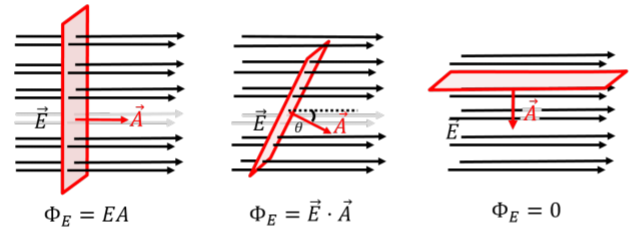
\includegraphics[width=12cm]{images/eflux.png}
\end{figure}

In cases where electric field is not uniform, we need to use the integral equation for electric flux:
\[ \dd{\Phi}_E = \vb{E}\cdot\dd{\vb{A}} \implies \Phi_E = \int \dd{\Phi_E} = \int \vb{E} \dd{\vb{A}} \]
where $\dd{\vb{A}}$ is the area vector perpendicular to the infinitesimally small surface, $\theta$ is the angle between $\vb{E}$ and $\dd{\vb{A}}$.

Total electric flux over any surface area is thus
\[ \Phi_E = \int_\text{surface}\vb{E}\cdot\dd{\vb{A}} \]

Typically total electric flux is evaluated over a closed surface. In such cases we replace the integral by
\begin{equation}
{\Phi_E \equiv \oint\vb{E}\cdot\dd{\vb{A}} = \oint E_n\dd{A}
}\end{equation}
where $E_n$ is the component of electric field strength normal to the surface.
\pagebreak

\begin{exmp}
Calculate the total electric flux through a spherical surface of radius $r$ with a charge $q$ located at its centre.
\end{exmp}

\begin{proof}[Solution]
Electric field strength at a distance $r$ from charge $q$ is
\[ \vb{E} = \frac{q}{4\pi\varepsilon_0r^2}\hat{\vb{r}} \]

Hence total electric flux is
\[ \Phi_E = \oint\frac{q}{4\pi\varepsilon_0r^2}\hat{\vb{r}}\cdot\dd{A} = \oint\frac{q}{4\pi\varepsilon_0r^2}\cdot\dd{A} = \frac{q}{4\pi\varepsilon_0r^2}4\pi r^2 = \frac{q}{\varepsilon_0} \]
\end{proof}
\pagebreak

\section{Gauss's Law}
For a point charge $q$ located at the centre of a sphere of radius $r$, magnitude of electric field everywhere on the surface of sphere is $\dfrac{k_eq}{r^2}$. We call the closed surface of the sphere a \textbf{gaussian surface} and the net electric flux through this surface is
\[ \Phi_E = \oint\vb{E}\cdot\dd{\vb{A}} = E\oint\dd{\vb{A}} \]
Using the expression for electric field and surface area of sphere, net flux through gaussian surface is 
\[ \Phi_E = \frac{q}{4\pi\varepsilon_0r^2}4\pi r^2 = \frac{q}{\varepsilon_0} \]

\begin{remark}
Net flux through any closed surface surrounding a point charge is independent of shape of that surface.

Net flux through a closed surface that surrounds no charge is zero.

Electric field due to many charges is the vector sum of electric fields produced by the individual charges.
\[ \oint\vb{E}\cdot\dd{\vb{A}} = \oint(\vb{E}_1+\vb{E}_2+\cdots)\cdot\dd{\vb{A}} \]
\end{remark}

Formally, 
\begin{thrm}{Gauss's Law}{}
Net flux through any closed surface surrounding a point charge $q$ is given by $\dfrac{q}{\varepsilon_0}$ and is independent of the shape of the surface.
\begin{equation}
{\Phi_E = \oint\vb{E}\cdot\dd{\vb{A}} = \frac{q_\text{in}}{\varepsilon_0}
}\end{equation}
\end{thrm}

\begin{figure}[H]
    \centering
    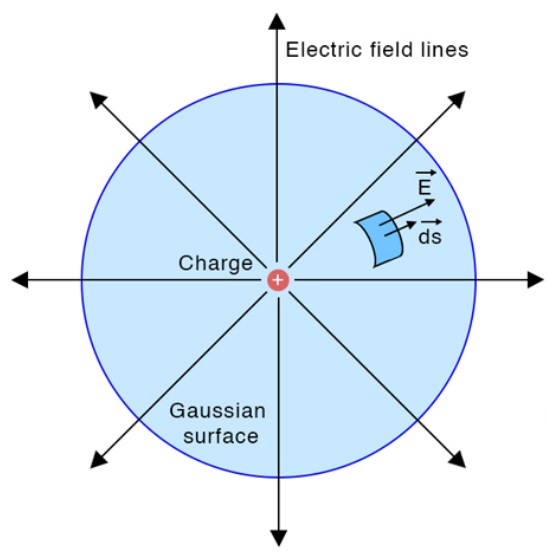
\includegraphics[width=8cm]{images/gauss_law_e.jpg}
\end{figure}

Conditions for Gauss's Law
\begin{itemize}
\item The surface must be closed.
\item The surface must pass through the point where the electric field is calculated.
\item The charge must be inside the surface.
\item The charge distribution must be continuous. The law cannot be applied to discrete charges.
\end{itemize}

Coulomb's Law derived from Gauss's Law:
\begin{proof}[Derivation]
Electric flux is given by
\[ \Phi_E = \oint\vb{E}\cdot\dd{\vb{A}} \]
If $\vb{E}$ and $\dd{\vb{A}}$ are parallel everywhere on the surface,
\[ \oint\vb{E}\cdot\dd{\vb{A}} = \oint E \dd{A} \]
For constant $E$ everywhere on the surface,
\[ \oint E \dd{A} = E \oint \dd{A}  \]
By Gauss's Law, 
\[ \Phi_E = E \oint \dd{A} = \frac{q_\text{in}}{\varepsilon_0} \]
Using surface area of a sphere,
\[ E(4\pi r^2) = \frac{q_\text{in}}{\varepsilon_0} \]
Hence electric field strength is given by
\[ E = \frac{q_\text{in}}{4\pi\varepsilon_0 r^2} \]
\end{proof}

\subsubsection{Conditions for gaussian surface}
Gauss's law can be used to determine electric fields in situations when the charge distribution is highly symmetric.

To determine a gaussian surface, we check whether each portion of the surface satisfies one or more of the following conditions:
\begin{itemize}
\item Value of electric field can be argued from symmetry to be constant over the surface.

Dot product of $\vb{E}\cdot\dd{\vb{A}}$ can be expressed as a simple algebraic product $E\dd{A}$ because the two vectors are \emph{parallel}.

\item Dot product of $\vb{E}\cdot\dd{\vb{A}}$ is 0 because the two vectors are \emph{perpendicular}.

\item Field is zero over the portion of the surface.
\end{itemize}
\pagebreak

\begin{exmp}
An insulating solid sphere of radius $a$ has a uniform volume charge density $\rho$ and carries a total positive charge $Q$.

Calculate the magnitude of the electric field at points outside and inside the sphere.
\end{exmp}
\begin{proof}[Solution] \ {\\}
\textbf{For a point outside solid sphere:}

As the solid has spherical symmetry, we choose a spherical gaussian surface of radius $r$, concentric with the solid sphere.
\[ \Phi_E = \oint\vb{E}\cdot\dd{\vb{A}} = \oint E\dd{A} = \frac{q_\text{in}}{\varepsilon_0} \]

Hence electric field strength is 
\[ E = \frac{Q}{4\pi\varepsilon_0r^2} = k_e\frac{Q}{r^2} \]

\textbf{For a point inside solid sphere:}

We choose a spherical gaussian surface of smaller radius than $a$. Charge $q_\text{in}$ within this gaussian surface by volume $V^\prime$ is less than $Q$.

By $q_\text{in}=\rho V^\prime$,
\[ q_\text{in} = \rho V^\prime = \frac{Q}{\frac{4}{3}\pi a^3}\frac{4}{3}\pi r^3 = \frac{Qr^3}{a^3} \]

Hence 
\[ \Phi_E = \oint\vb{E}\cdot\dd{\vb{A}} = \oint E\dd{A} = \frac{q_\text{in}}{\varepsilon_0} \]
\[ E = \frac{q_\text{in}}{4\pi\varepsilon_0r^2} = k_e\frac{Q}{a^3}r \]
\end{proof}
\pagebreak

\section{Conductors in electrostatic equilibrium}
\begin{defn}{Electric conductors}{}
Materials in which some of the electrons are free electrons that are not bound to atoms and can move relatively freely under the influence of an applied electric field.
\end{defn}

When there is no net motion of charge within a conductor, the conductor is in electrostatic equilibrium. A conductor in electrostatic equilibrium has the following properties:

\begin{itemize}
\item 
\end{itemize}

\section{Electric dipole}
\begin{defn}{Electric dipole}{}
An electric dipole consists of two equal but opposite charges, $+q$ and $-q$, separated by a distance $2a$.
\end{defn}

Dipole moment vector is given by 
\begin{equation}
{\vb{p} = 2qa\hat{\vb{r}}
}\end{equation}
where $2a$ is the distance between the charges. $\vb{p}$ points from the negative to the positive charge.
\[ |\vb{p}| = 2qa \]

Like individual charges, dipoles both create electric fields and respond to them. When placed in an external field, a dipole will attempt to rotate in order to align with the field, and, if the field is non-uniform in strength, will experience a force as well. 

\subsection{Electric Field of a Dipole}

\subsection{Dipole in Electric Field}
\begin{figure}[H]
    \centering
    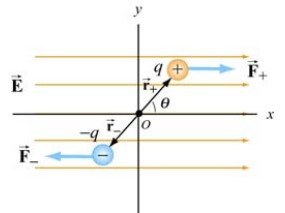
\includegraphics[width=8cm]{images/dipole_in_e_field.jpg}
\end{figure}

When an electric dipole is placed in a uniform external electric field $\vb{E}$ and makes angle $\theta$ with the field, torque $\tau$ is produced.

Torque $\tau$ is the cross product of vectors $\vb{p}$ and $\vb{E}$.
\begin{equation}
{\tau = \vb{p} \times \vb{E}
}\end{equation}

Magnitude of torque is given by
\[ \tau = pE\sin\theta \]



\subsection{Potential Energy of an Electric Dipole}


\pagebreak

\chapter{Magnetic Fields}
Magnetic B-field; Lorentz force; Ampère’s force; Biot-Savart law and B-field on the axis of a circular current loop and for simple symmetric systems like straight wire, circular loop and long solenoid.



\section{Magnetic Field}
Magnetic fields (or ``B" fields) are be created by magnetic dipoles. Just like electric charges are described as positive and negative charges, magnetic poles are described as north and south poles.\footnote{A magnetic monopole has never been found. This does not mean magnetic monopoles do not exist. We cannot prove magnetic monopoles do not exist; we can only say we have no evidence that they exist.}

A permanent magnet produces a special field around the magnet in which magnetic forces act. This field is called a \textbf{magnetic field} whose direction is the N-pole direction of a compass. 

An electric current produces a magnetic field that points clockwise around the current. If a current flows through a solenoid, a magnetic field that passes through the solenoid and points in the rightward direction is produced. 

The curves drawn to represent a magnetic field are called \textbf{magnetic field lines}. Magnetic field lines point outward from the N-pole of a permanent magnet and point inward to the S-pole; they neither disappear nor intersect one another.

Just like materials have an electric permittivity $\varepsilon$, materials also have a magnetic permeability $\mu$. Magnetic permeability is the measurement of the amount of magnetisation a material has in response to an external magnetic field. Magnetic permeability of free space has a constant value $\mu_0 = 4\pi \times 10^{-7}$ \unit{T.m.A^{-1}}.


\section{Magnetic Force on Current}
A magnetic field exerts a force on a current. If the magnetic field is in the direction of the index finger of a left hand and the current is in the direction of the middle finger, then the force on the current is in the direction of the thumb. This rule is called \textbf{Fleming’s left-hand rule}.

\begin{figure}[H]
    \centering
    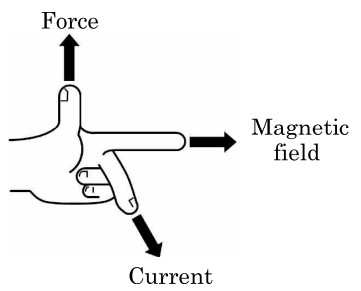
\includegraphics[width=8cm]{images/fleming_lhr.jpg}
\end{figure}

A magnetic field is defined by the fact that a moving electric charge in a B field can experience a magnetic force, $\vb{F}_B$.
\begin{equation}
{\vb{F}_B = 
}\end{equation}

\section{Electromagnetic Induction}
\textbf{Electromagnetic induction} is a phenomenon where an e.m.f. is induced when the number of magnetic field lines through the coil vary with time. The emf is induced to prevent the change in the magnetic field lines through the coil, and its magnitude is proportional to the instantaneous rate of change of the magnetic field lines through the coil.

\begin{thrm}{Biot-Savart law}{}
Magnetic field due to a long straight wire is
\begin{equation}
{B=\frac{\mu_{0} N I}{2 R}
}\end{equation}
\end{thrm}

\section{Ampere's Law}
We consider a straight conductor carrying a current of $I$. The magnitude of the magnetic field, $B$, on the circumference of radius $r$ in a plane perpendicular to the conductor is
\[ B \cdot 2\pi r = \mu_0I. \]
That is, the product of the length of the circumference and $B$ is equal to $\mu_0I$.




\begin{thrm}{Amp\`{e}re's law}{}
Line integral of $\vb{B}\cdot\dd{\vb{s}}$ around any closed path equals to $\mu_0I$, where $I$ is the total current passing through any surface bounded by the closed path:
\begin{equation}
{\oint \vb{B}\cdot\dd{\vb{s}} = \mu_0I}
\end{equation}
\end{thrm}

\begin{exmp}
A long straight wire of radius $R$ carries a steady current $I$ that is uniformly distributed through the cross-section of the wire.

Calculate the magnetic field at a distance $r$ from the centre of the wire in the regions $r\ge R$ and $r\le R$.
\end{exmp}

\section{Lorentz force}
In a uniform magnetic field of magnitude $B$, the magnitude of the magnetic force, $F$, that acts on a point charge of $q$ moving perpendicularly to the magnetic field at a speed of $v$ is
\[ F=Bqv \]



\section{Electromagnetic Induction and Self-Inductance}

\section{}


Gauss’ law (for E- and B-fields); Ampère’s law; Faraday’s law; using these laws for the calculation of fields when the integrand is almost piece-wise constant. 

Boundary conditions for the electric field (or electrostatic potential) at the surface of conductors and at infinity; concept of grounded conductors. 
Superposition principle for electric and magnetic fields; uniqueness of solution to well-posed problems; method of image charges.
\pagebreak

\chapter{Interaction of matter with electric and magnetic fields}
Resistivity and conductivity; differential form of Ohm’s law. 
Dielectric and magnetic permeability; relative permittivity and permeability of electric and magnetic materials; energy density of electric and magnetic fields; ferromagnetic materials; hysteresis and dissipation; eddy currents; Lenz’s law. 
Charges in magnetic field: helicoidal motion, cyclotron frequency, drift in crossed E- and B-fields. 
Energy of a magnetic dipole in a magnetic field; dipole moment of a current loop.
\pagebreak

\chapter{Circuits}
Linear resistors and Ohm’s law; Joule’s law; work done
by an electromotive force; ideal and non-ideal batter-
ies, constant current sources, ammeters, voltmeters and
ohmmeters. Nonlinear elements of given V -I characteristic. 

\chapter{Capacitors and Inductors}
\section{Capacitance and inductance}
\textbf{Capacitors} are used to store energy in electrical and electronic circuits. 

Every capacitor has two leads, each connected to a metal plate. To store energy, these two plates must be given equal and opposite electric charges. Between the plates is an insulating material called the \textbf{dielectric}.

Applying a potential difference to the plates of a capacitor causes electrons to move to or from the plates. Electrons are removed from one plate, and an equal number of electrons are added to the other plate.

\begin{figure}[H]
    \centering
    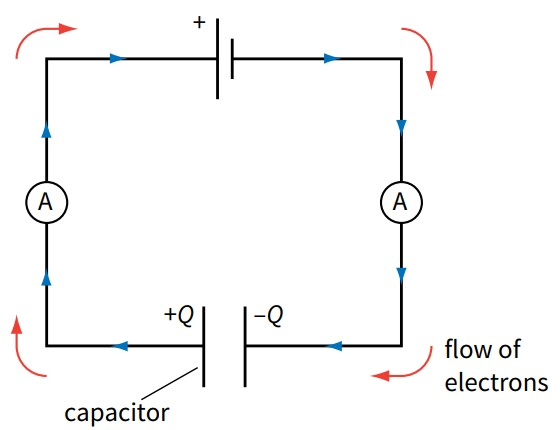
\includegraphics[width=8cm]{images/capacitor.jpg}
\end{figure}

\begin{defn}{Capacitance}{}
Ratio of the change in electric charge on either conductor of a capacitor to the change in potential difference between them.
\begin{equation}
{C \equiv \frac{Q}{V}
}\end{equation}
\end{defn}

\[ C=k\varepsilon_0\frac{A}{d} \]
where $k$ depends on the material between the plates.

An \textbf{inductor} is a passive component used to store energy in the form of magnetic energy when electricity is applied to it. One of the key properties of an inductor is that it impedes or opposes any change in the amount of current flowing through it.

\begin{defn}{Self-inductance}{}
Ratio of the e.m.f. induced in an electrical circuit or component to the rate of change of current causing it.
\[ V = L \dv{I}{t} \]
\end{defn}

\begin{defn}{Mutual inductance}{}
Tendency of an electrical circuit or component to oppose a change in the current in a nearby electrical circuit or component.
\end{defn}

\section{Dielectrics and ferromagnetic materials}
\begin{defn}{Dielectric material}{}
Dielectric materials enhance capacitance by allowing the electric field between the plates to induce charge dipoles in it, thus increasing the ability of the capacitor to store energy; dielectric breakdown can occur when the electric field is sufficiently strong, where a conducting path between the plates is formed and charge jumps across the gap, usually destroying the capacitor.
\end{defn}

\begin{defn}{Ferromagnetic material}{}
Ferromagnetic materials enhance inductance by allowing the magnetic field within the inductor to align its domains, thus increasing the ability of the inductor to store energy; this enhancement is non-linear as the magnetic field due to the current increases, especially near saturation where the intrinsic magnetic dipole moments within the material are almost aligned perfectly with the field and cannot be further aligned to produce still higher magnetisation.
\end{defn}

\section{Energy in a capacitor and in an inductor}
\begin{figure}[H]
    \centering
    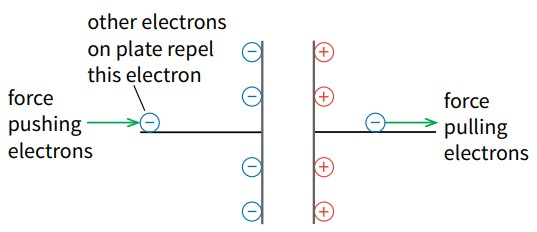
\includegraphics[width=8cm]{images/capacitor_energy.jpg}
\end{figure}

Energy stored in capacitor:
\begin{equation}
{U = \frac{1}{2}CV^2 = \frac{1}{2}QV
}\end{equation}

\begin{proof}
Potential energy stored in a capacitor $U$ is equal to the work done $W$ by a battery with potential difference $V$ to put a charge $Q$ on a capacitor with capacitance $C$.

Work done on a charge against an element of potential difference in the battery is given by $\dd{W} = Q \dd{V}$.

From the definition of capacitance, 
\[ C = \frac{Q}{V} \implies Q = CV \]

Thus 
\[ \dd{U} = \dd{W} = Q \dd{V} \implies U = \int_0^V CV \dd{V} = \frac{1}{2}CV^2 \]
\end{proof}

Potential energy stored in an inductor is 
\begin{equation}
{U = \frac{1}{2}LI^2
}\end{equation}

\begin{proof}
The potential energy stored in an inductor $U$ is equal to the work done $W$ by a battery to move a charge $Q$ through the inductor.

Work done on an element of charge against the potential difference in a battery is $\dd{W} = V \dd{Q}$.

From the definition of inductance, \[ V = L \dv{T}{t} \]

Thus 
\[ \dd{U} = \dd{W} = L\dv{I}{t}\dd{Q} = LI\dv{Q}{t} \dd{I} \implies U = \int_0^I LI \dd{I} = \frac{1}{2}LI^2 \]
\end{proof}


\section{Circuits with capacitors and inductors}
Capacitors arranged in series: (common charge on capacitors)
\[ \frac{1}{C_T} = \sum_i\frac{1}{C_i} \]

Capacitors arranged in parallel: (common p.d. across capacitors)
\[ C_T = \sum_iC_i \]

Inductors in series (common rate of change of current through inductors)
\[ L_T = \sum_iL_i \]

Inductors in parallel (common self-induced e.m.f. across inductors)
\[ \frac{1}{L_T} = \sum_i\frac{1}{L_i} \]





Capacitors and capacitance (also for a single electrode with respect to infinity); self-induction and inductance; energy of capacitors and inductors; mutual inductance; time constants for RL and RC circuits. 

\chapter{Inductors}


\chapter{AC circuits}
AC
circuits: complex amplitude; impedance of resistors, in-
ductors, capacitors, and combination circuits; phasor di-
agrams; current and voltage resonance; active power.


\part{Quantum Physics}
\chapter{Probability waves}
Particles as waves: relationship between the frequency and energy, and between the wave vector and momentum. energy levels of hydrogen-like atoms (circular orbits only) and of parabolic potentials; quantisation of angular momentum.
Uncertainty principle for the conjugate pairs of time and energy, and of coordinate and momentum (as a theorem, and as a tool for estimates);
\pagebreak

\chapter{Structure of matter}
Emission and absorption spectra for hydrogen-like atoms (for other atoms — qualitatively), and for molecules due to molecular oscillations; spectral width and lifetime of excited states. Pauli exclusion principle for Fermi particles. Particles (knowledge of charge and spin): electrons, electron neutrinos, protons, neutrons, photons; Compton scattering. Protons and neutrons as compound particles. Atomic nuclei, energy levels of nuclei (qualitaively); alpha-, beta- and gamma-decays; fission, fusion and neutron capture; mass defect; half life and exponential decay. photoelectric effect.


\part{Thermodynamics}
\chapter{Classical thermodynamics}
\section{The zeroth law of Thermodynamics}
Concepts of thermal equilibrium and reversible pro-
cesses; internal energy, work and heat; Kelvin’s tem-
perature scale; entropy; open, closed, isolated systems;
first and second laws of thermodynamics. Kinetic the-
ory of ideal gases: Avogadro number, Boltzmann factor
and gas constant; translational motion of molecules and
pressure; ideal gas law; translational, rotational and os-
cillatory degrees of freedom; equipartition theorem; in-
ternal energy of ideal gases; root-mean-square speed of
molecules. Isothermal, isobaric, isochoric, and adiabatic
processes; specific heat for isobaric and isochoric pro-
cesses; forward and reverse Carnot cycle on ideal gas and
its efficiency; efficiency of non-ideal heat engines.

Equation of state
\begin{equation}
pV = nRT
\end{equation}
where $n$ is the amount of substance in moles, $R = 8.31$ \unit{J.K^{-1}.mol^{-1}} is the molar gas constant. $N_A = 6.02 \times 10^{23}$ \unit{mol^{-1}} is the Avogardo number.

This equation can also be written as
\[ pV = Nk_BT \]
where $k_B = \frac{R}{N_A} = 1.38 \times 10^{-23}$ \unit{J.K^{-1}} is the Boltzmann constant.

\begin{thrm}{0th Law of Thermodynamics}{}
If A, B and C are different thermodynamical systems and A is in thermodynamical equilibrium with B and B is in thermodynamical equilibrium with C, then A is in thermodynamical equilibrium with C.
\end{thrm}

\section{The first law of Thermodynamics}
We saw from the zeroth law that there are two kinds of energy that can be transferred between a thermodynamical system and its surroundings:
\begin{enumerate}
\item work $W$ by mechanical contact
\item heat $Q$ by thermal contact
\end{enumerate}

\begin{thrm}{1st Law of Thermodynamics}{}
The internal energy of an isolated system is conserved under any thermodynamical change.

Under any thermodynamical change,
\begin{equation}
U = Q + W
\end{equation}
\end{thrm}

where $U$ is the internal energy of the system (function of state),$ $Q is heat added to the system, $W$ is the work done \emph{on} the system.

According to the first law we thus have $Q_\text{surr} = Q$ and $W_\text{surr} = W$, where the subscript ``surr" indicates the system’s surroundings.

\subsection{Internal energy}
The energy $E_l$ of a particle $l$, according to the fundamental laws of physics, is either in kinetic or potential form, which we will write $E_{l,K}$ and $E_{l,P}$ respectively. 

We introduce an internal state energy $E_{l,I}$, which is composed of intra-molecular kinetic and potential energies reflecting the structure of the molecule.

So the total internal energy of a system is simply
\[ E = \sum_l (E_{l,K} + E_{l,P} + E_{l,I}) \]

\pagebreak

\chapter{Heat transfer and phase transitions}
Phase transitions (boiling, evaporation, melting, sublimation) and latent heat; saturated vapour pressure, relative humidity; boiling; Dalton’s law; concept of heat conductivity; continuity of heat flux.

Thermal conduction:
\begin{thrm}{Fourier's Law}{}
\begin{equation}
{\frac{Q}{t} = \frac{kA\Delta T}{L}
}\end{equation}
where $\frac{Q}{t}$ is rate of thermal energy transfer, $k$ is thermal conductivity, $A$ is barrier cross-sectional area, $\Delta T$ is temperature difference, $L$ is barrier thickness.
\end{thrm}
\pagebreak


\part{Statistical physics}
Planck’s law, Wien’s displacement law; the Stefan-Boltzmann law.



\end{document}